%!TEX root = ../my_thesis.tex
\section{Decay-time fit validation with bootstrapping}
\label{app:mcbootstrap}

In this appendix, further results of the Monte Carlo time fit validation are shown in addition to Fig.~\ref{fig:mc_bootstrap_cp}. The results for the production asymmetry, detection asymmetry, and acceptance parameters are not shown because no independent reference value for these parameters exists in Monte Carlo.
\begin{figure}[htpb]
        \begin{center}
                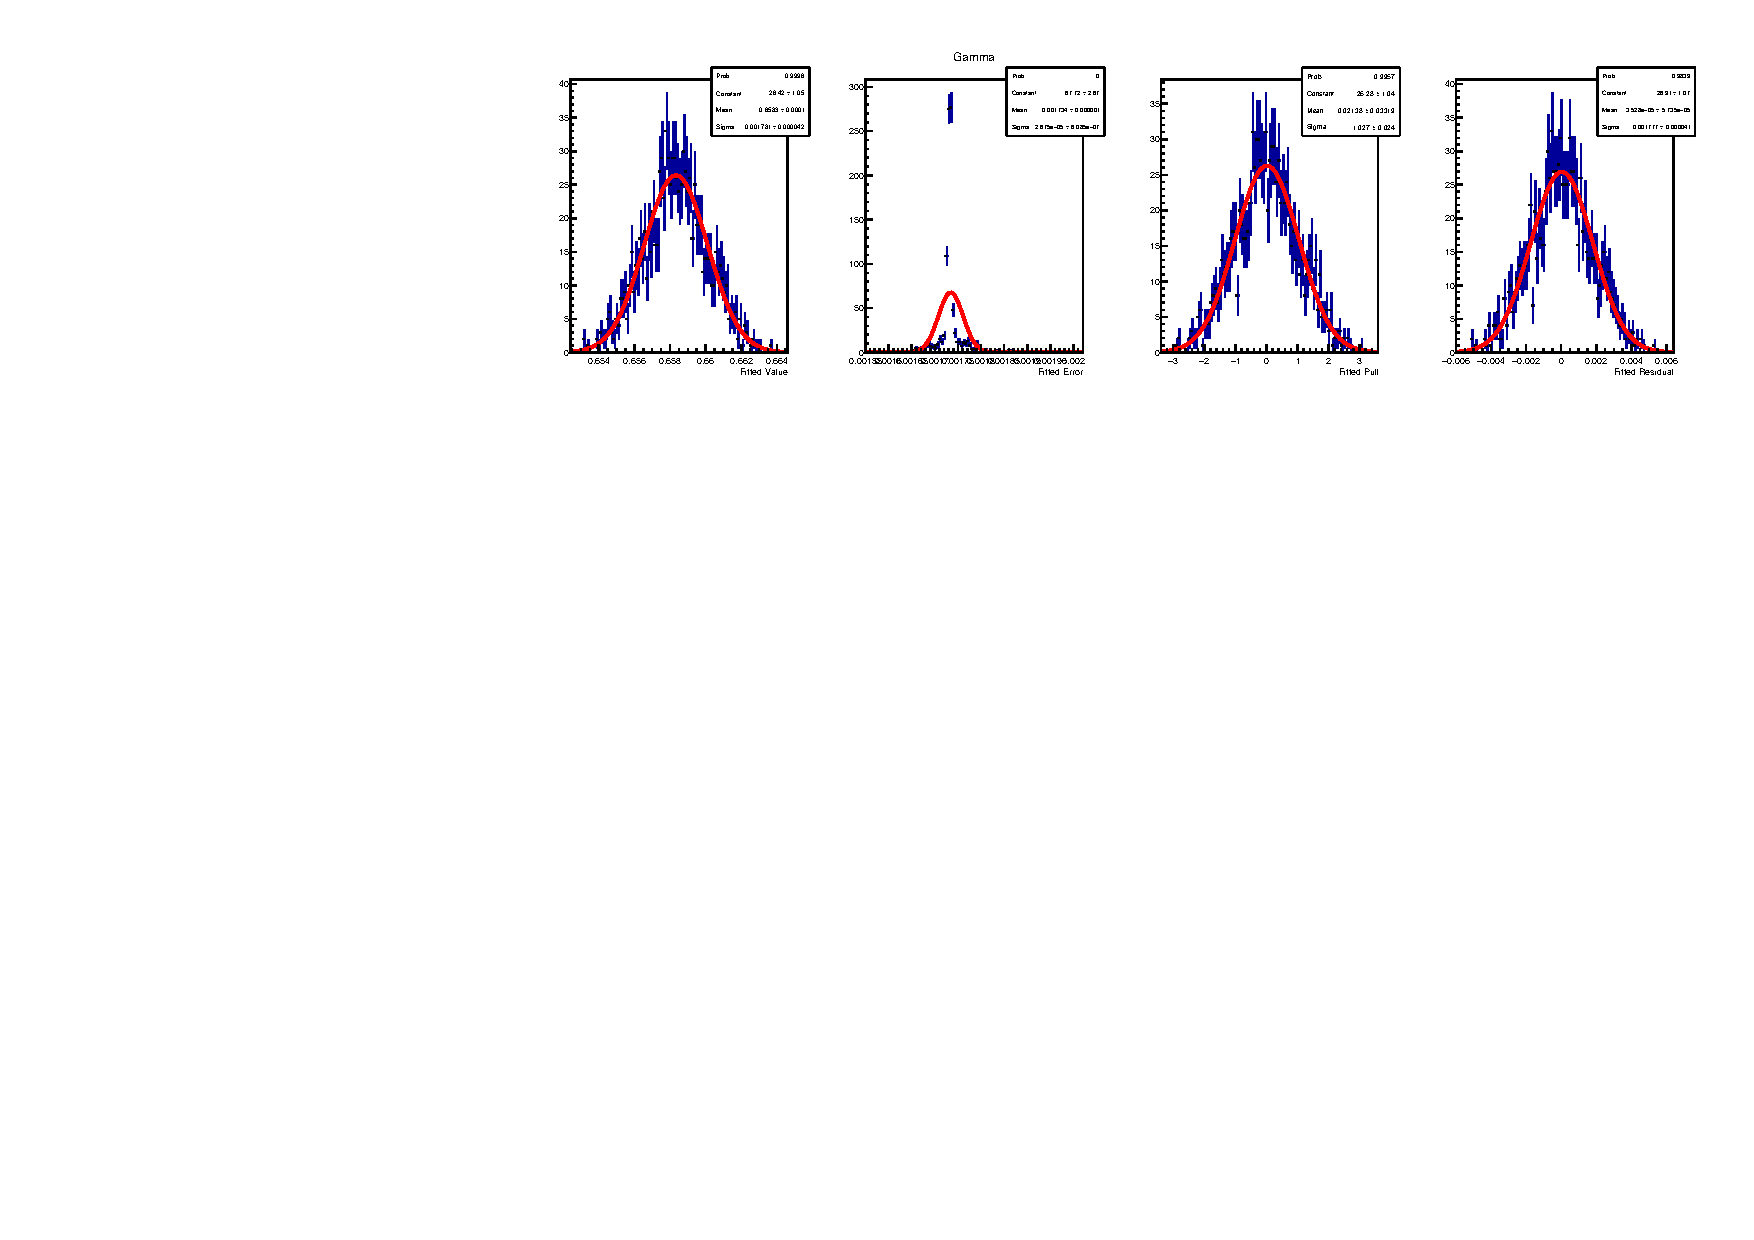
\includegraphics[width=0.9\textwidth]{AA-Appdx-mcbootstrap/figs/1DPullPlot_Gamma_SSbarAccAsymmFTFloatDMGammaConstrAllSamples.pdf} \\
                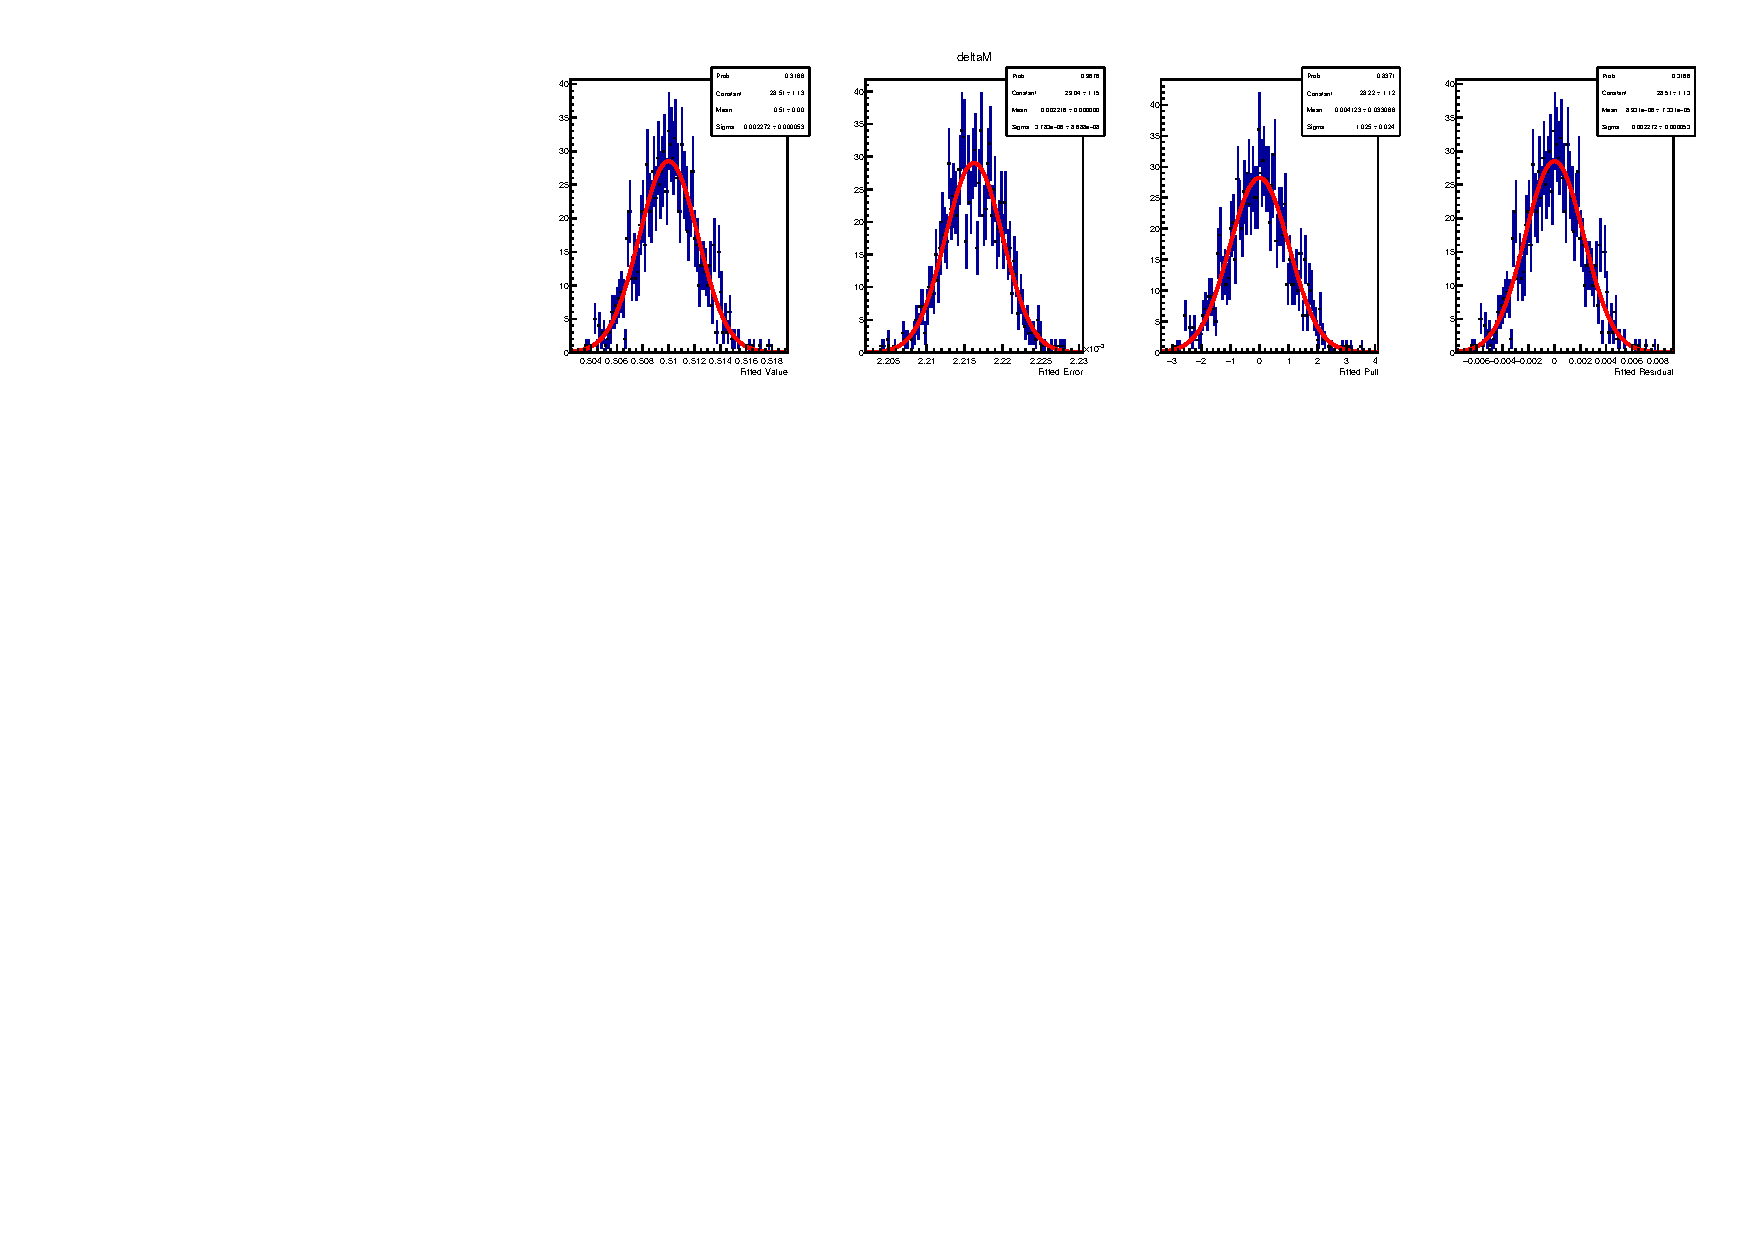
\includegraphics[width=0.9\textwidth]{AA-Appdx-mcbootstrap/figs/1DPullPlot_deltaM_SSbarAccAsymmFTFloatDMGammaConstrAllSamples.pdf}
        \end{center}
        \vspace{-2mm}
        \caption{Distributions of the fitted value, error, pull and residual for $\Gamma$ (top) and $\Delta m$ (bottom). Each distribution is fitted with a Gaussian function. The result of the Gaussian fit is shown for the fitted error as well, even though uncertainties are not always Gaussian. Pulls and residuals are computed by taking the Monte Carlo generation value as reference (see Appendix~\ref{app:mcgen}).}
        \label{fig:mc_bootstrap_decay}
\end{figure}

\begin{figure}[t]
  \begin{center}
    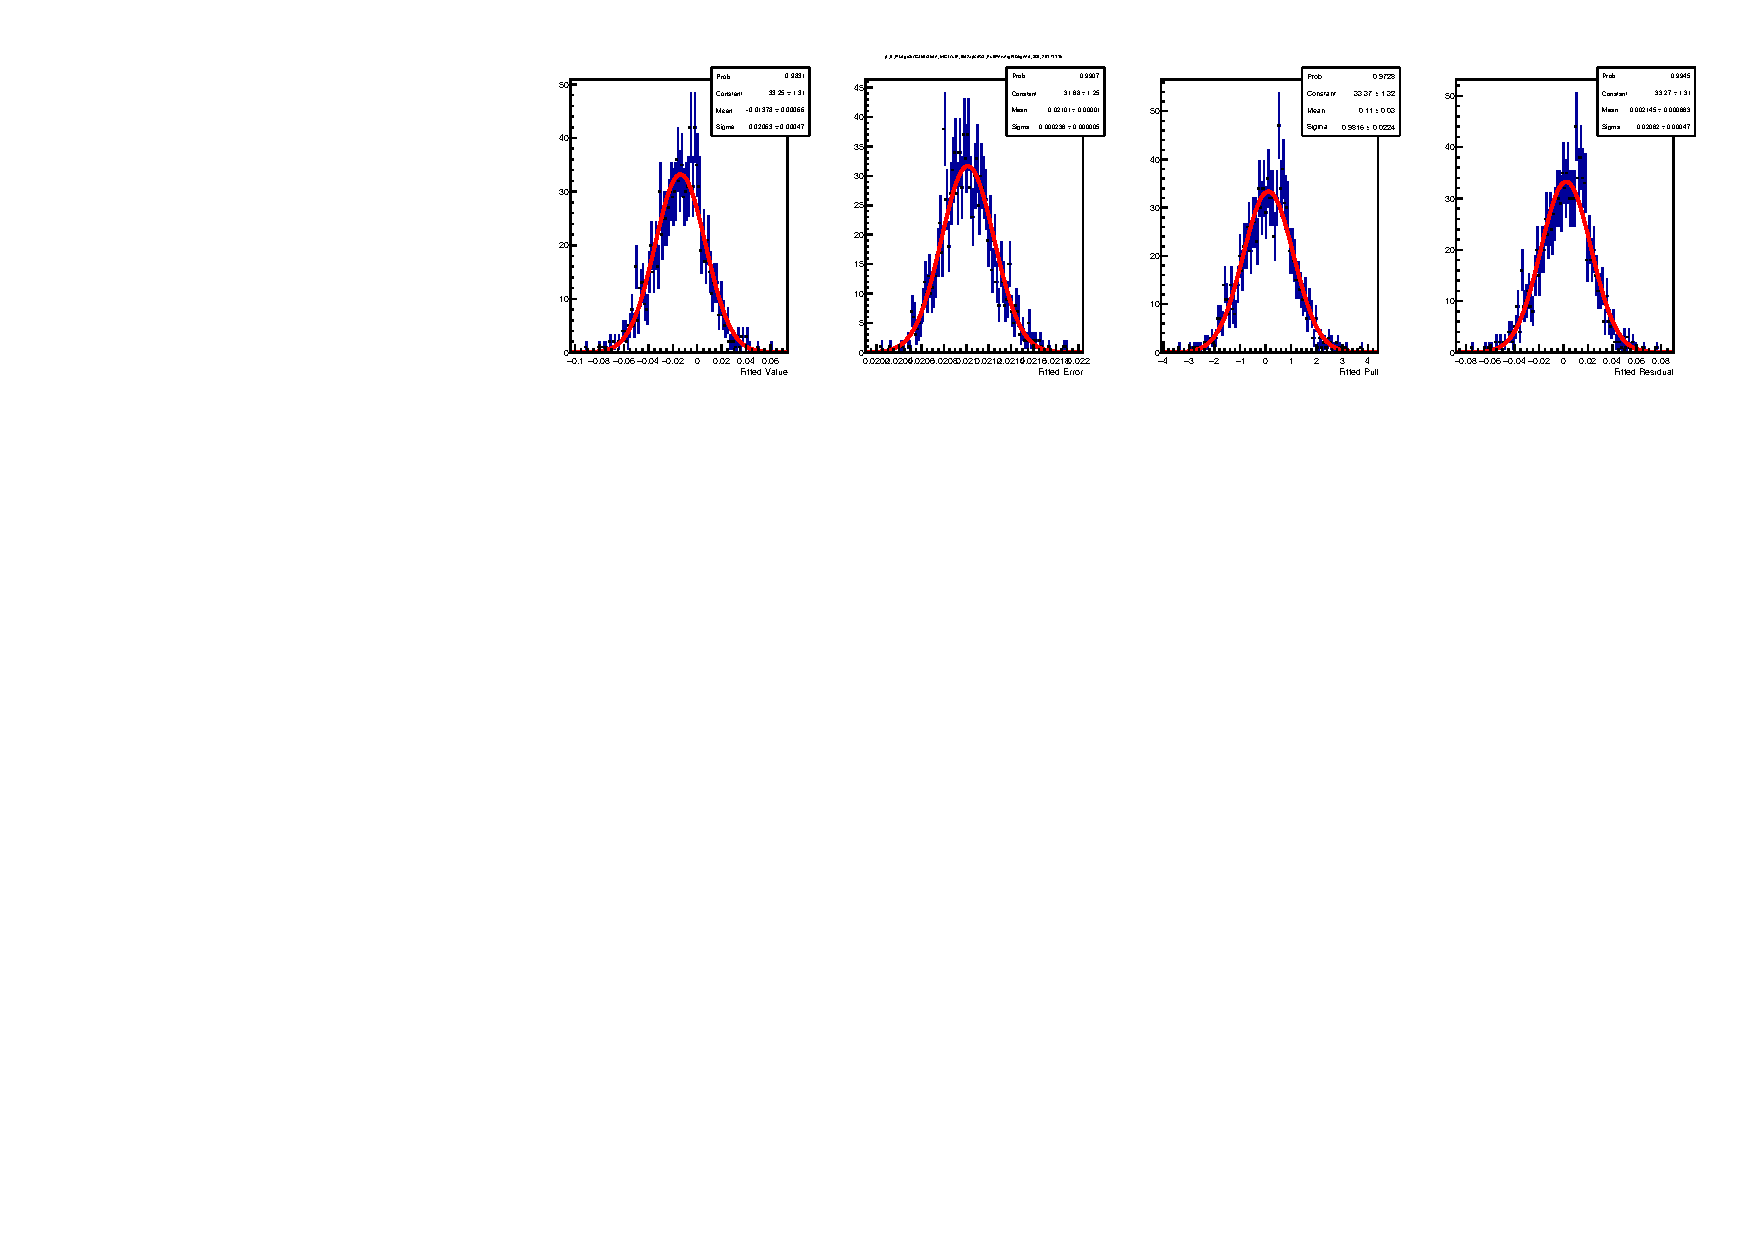
\includegraphics[width=0.9\textwidth]{AA-Appdx-mcbootstrap/figs/1DPullPlot_p_0_RLogisticCalibration_MCTruth_Bd2JpsiKst_FullReweightAligned_SS_20171116_SSbarAccAsymmFTFloatDMGammaConstrAllSamples.pdf} \\
    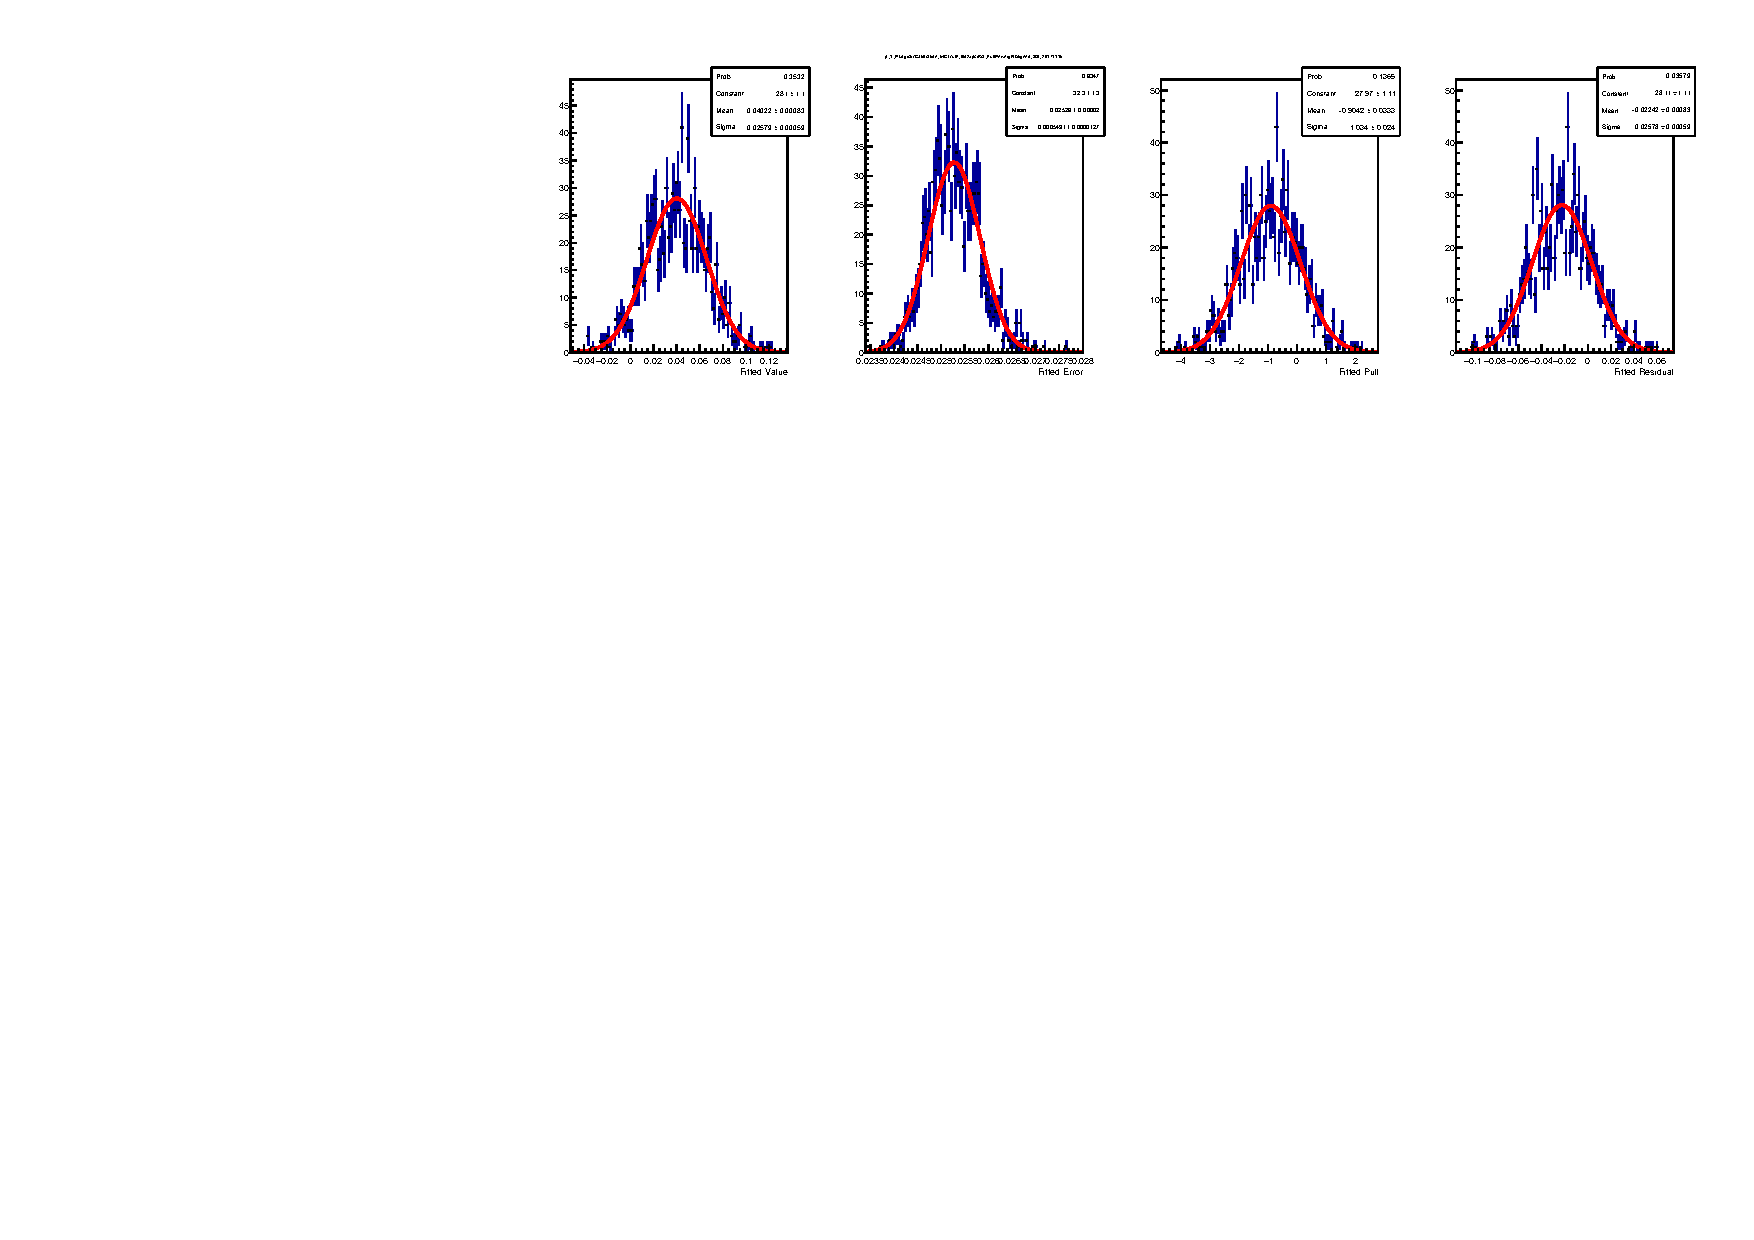
\includegraphics[width=0.9\textwidth]{AA-Appdx-mcbootstrap/figs/1DPullPlot_p_1_RLogisticCalibration_MCTruth_Bd2JpsiKst_FullReweightAligned_SS_20171116_SSbarAccAsymmFTFloatDMGammaConstrAllSamples.pdf} \\
    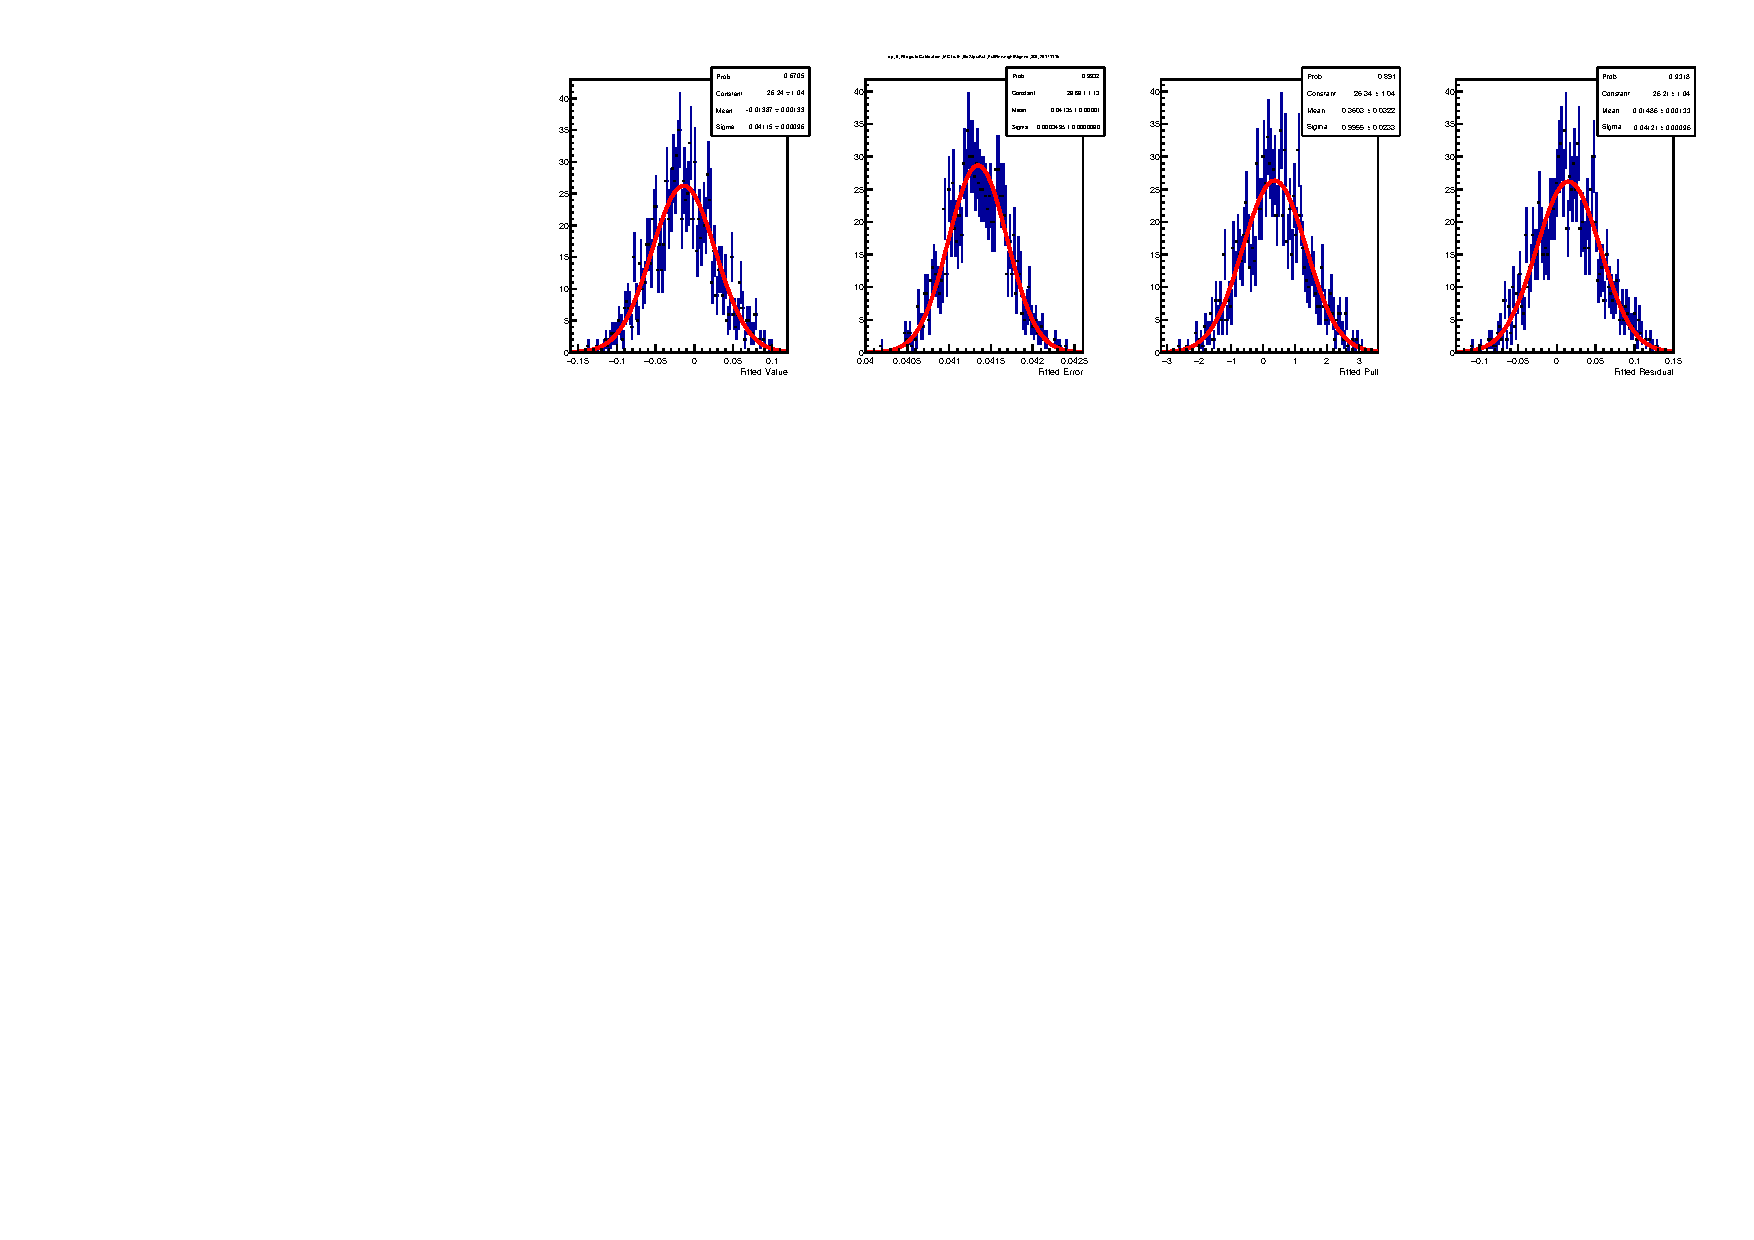
\includegraphics[width=0.9\textwidth]{AA-Appdx-mcbootstrap/figs/1DPullPlot_dp_0_RLogisticCalibration_MCTruth_Bd2JpsiKst_FullReweightAligned_SS_20171116_SSbarAccAsymmFTFloatDMGammaConstrAllSamples.pdf} \\
    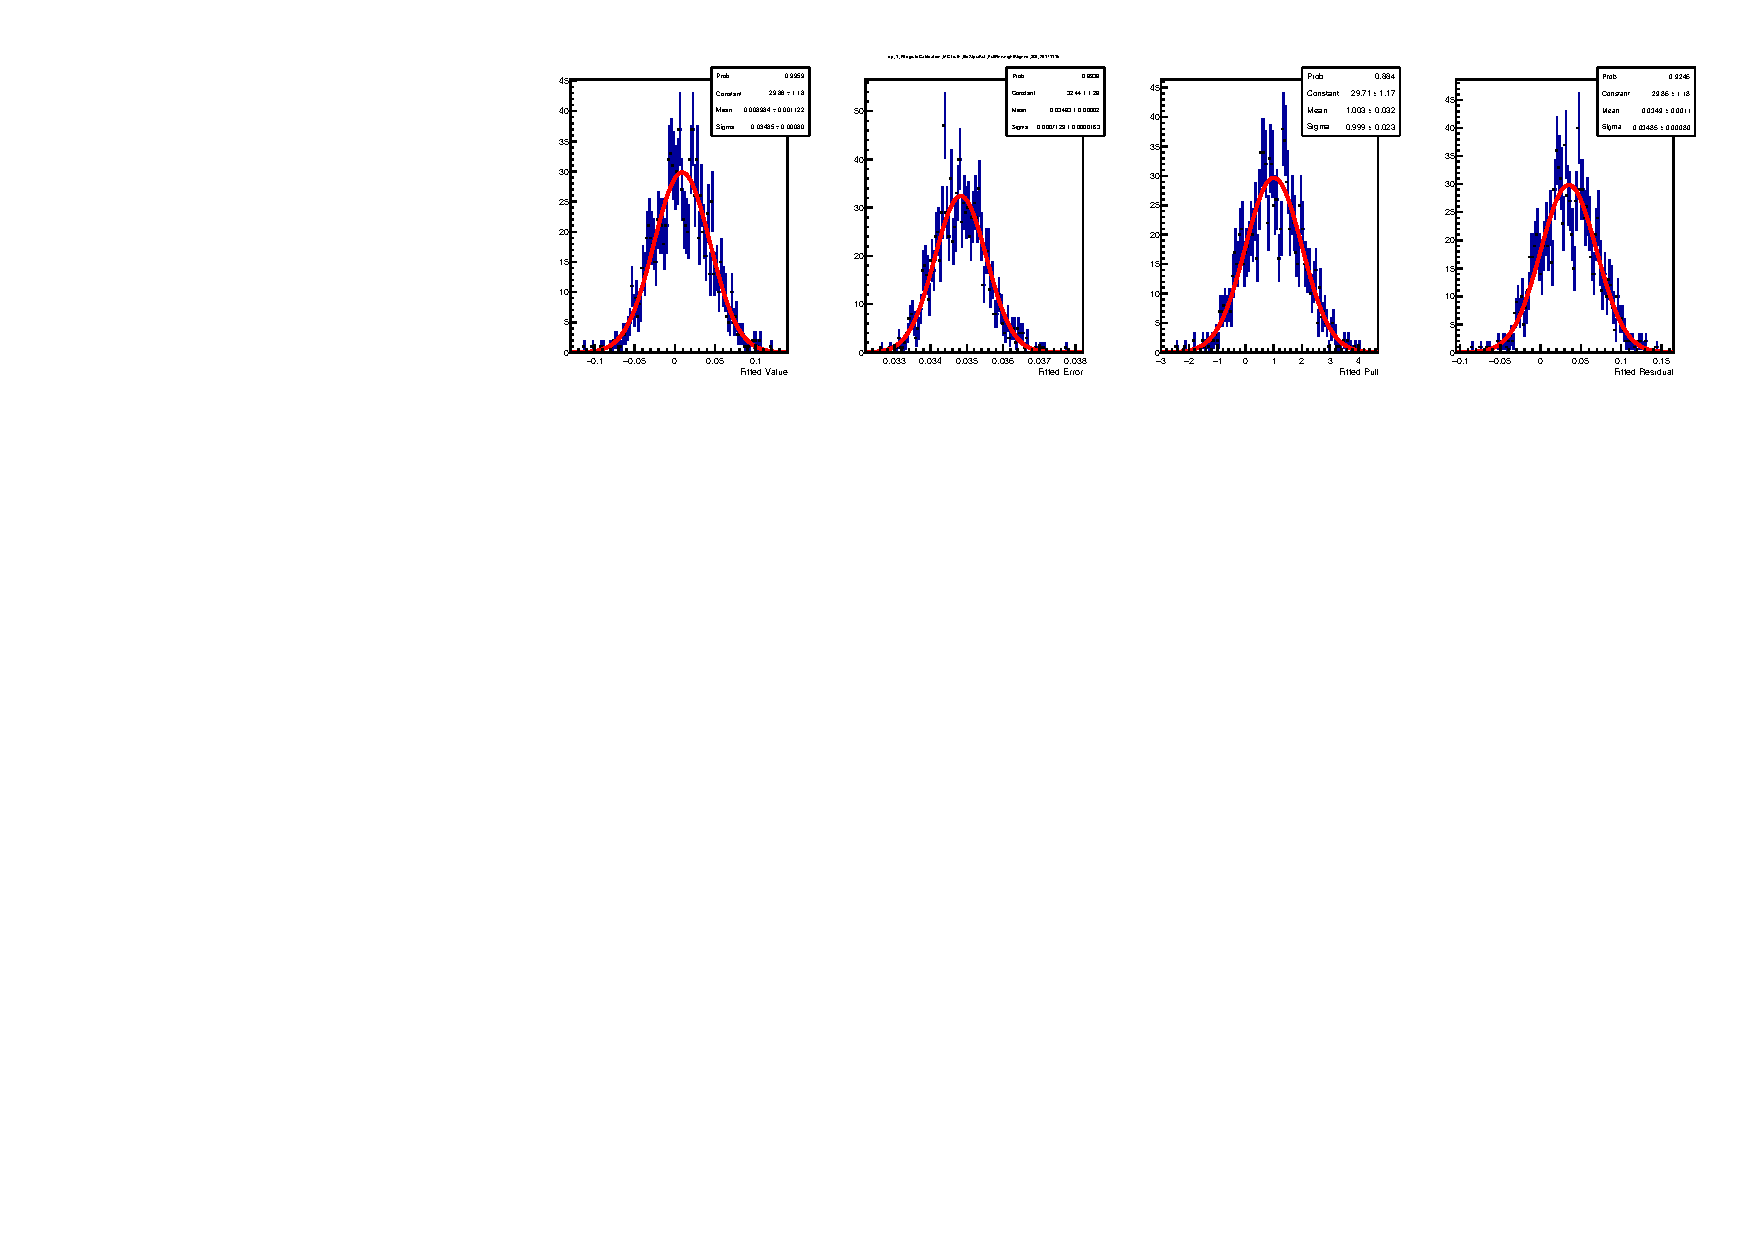
\includegraphics[width=0.9\textwidth]{AA-Appdx-mcbootstrap/figs/1DPullPlot_dp_1_RLogisticCalibration_MCTruth_Bd2JpsiKst_FullReweightAligned_SS_20171116_SSbarAccAsymmFTFloatDMGammaConstrAllSamples.pdf}
  \end{center}
  \vspace{-2mm}
  \caption{Distributions of the fitted value, error, pull and residual for the SS tagger calibration parameters $p_0^{\rm SS}$, $p_1^{\rm SS}$, $\Delta p_0^{\rm SS}$, and $\Delta p_1^{\rm SS}$ (from top to bottom). Each distribution is fitted with a Gaussian function. The result of the Gaussian fit is shown for the fitted error as well, even though uncertainties are not always Gaussian. Pulls and residuals are computed by taking the values found on the $\Bz\to\jpsi\Kstarz$ Monte Carlo calibration as reference (see Table~\ref{tab:ss_calib_portability_mc}).}
  \label{fig:mc_bootstrap_ss}
\end{figure}

\begin{figure}[t]
  \begin{center}
    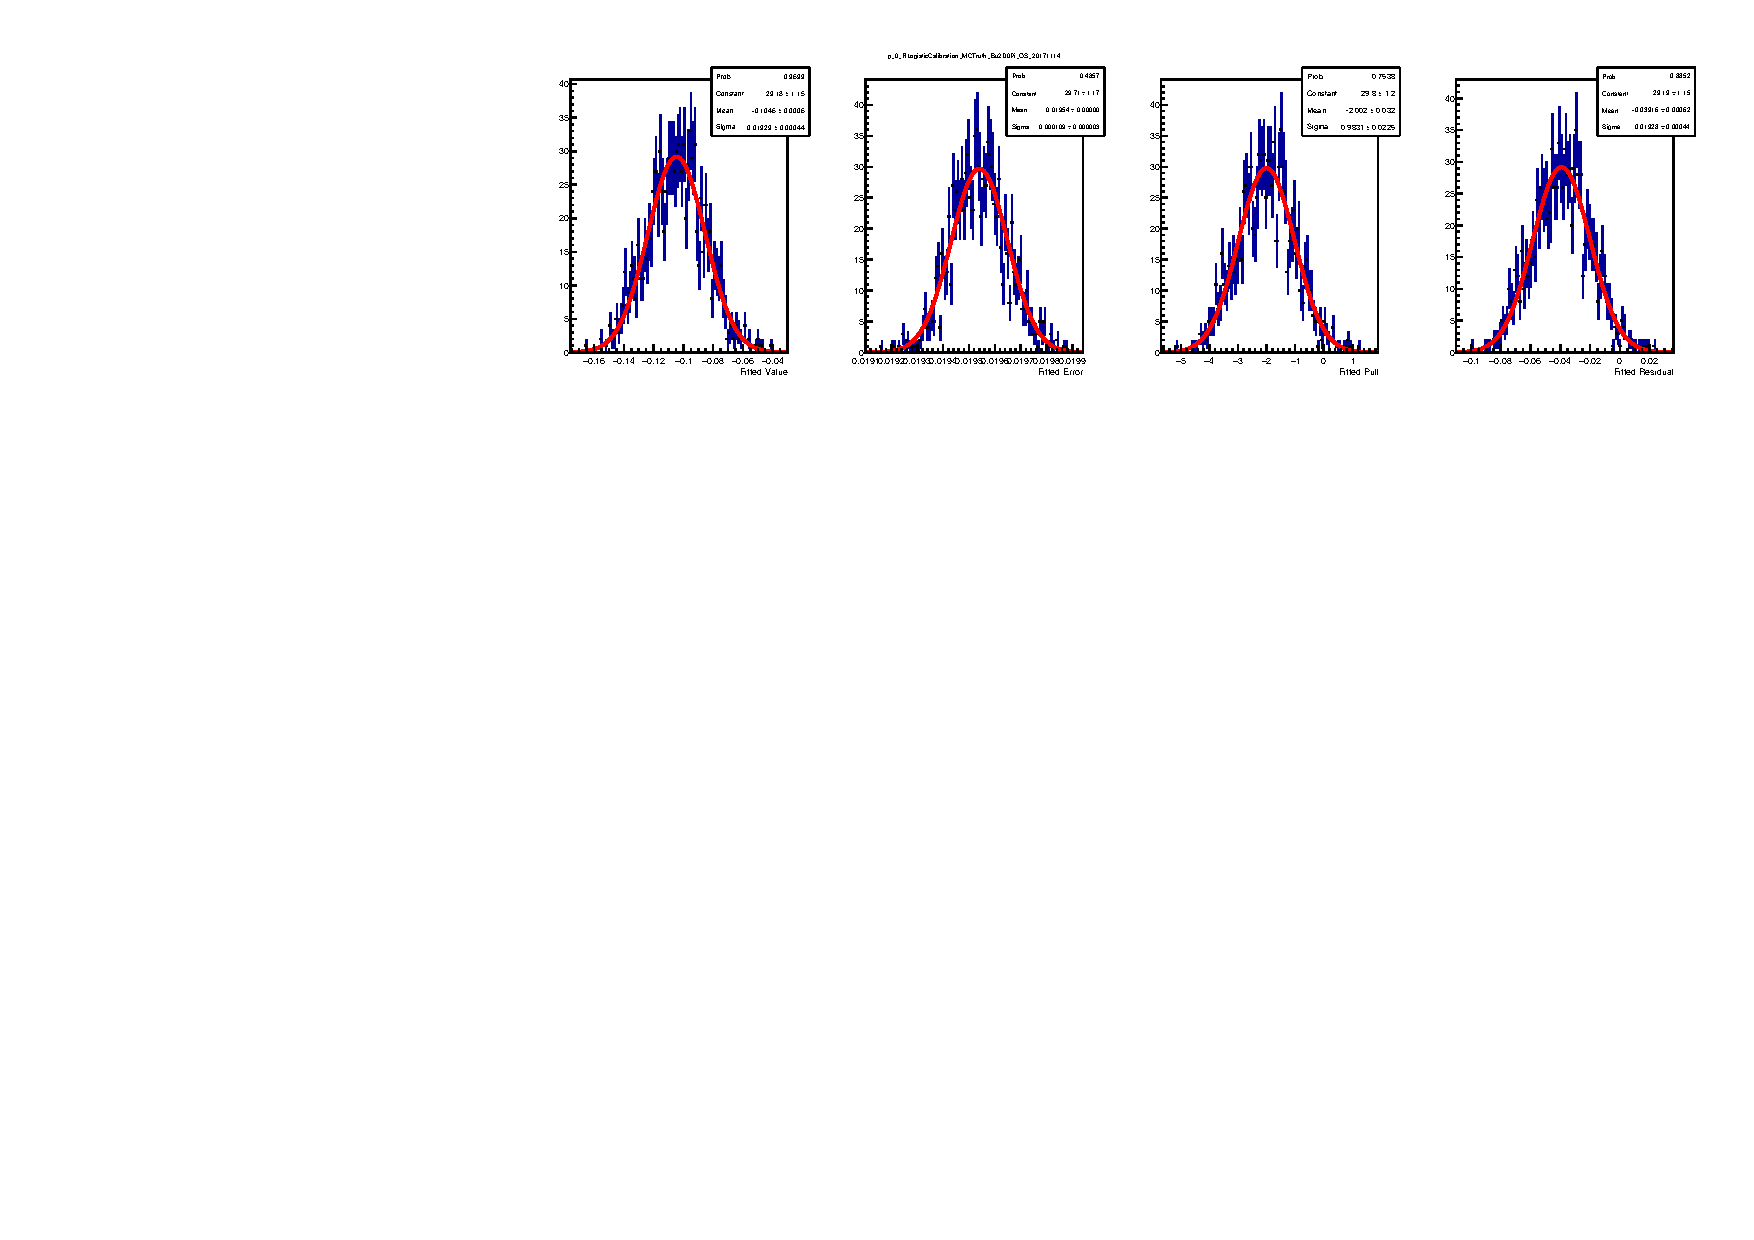
\includegraphics[width=0.8\textwidth]{AA-Appdx-mcbootstrap/figs/1DPullPlot_p_0_RLogisticCalibration_MCTruth_Bu2D0Pi_OS_20171114_SSbarAccAsymmFTFloatDMGammaConstrAllSamples.pdf} \\
    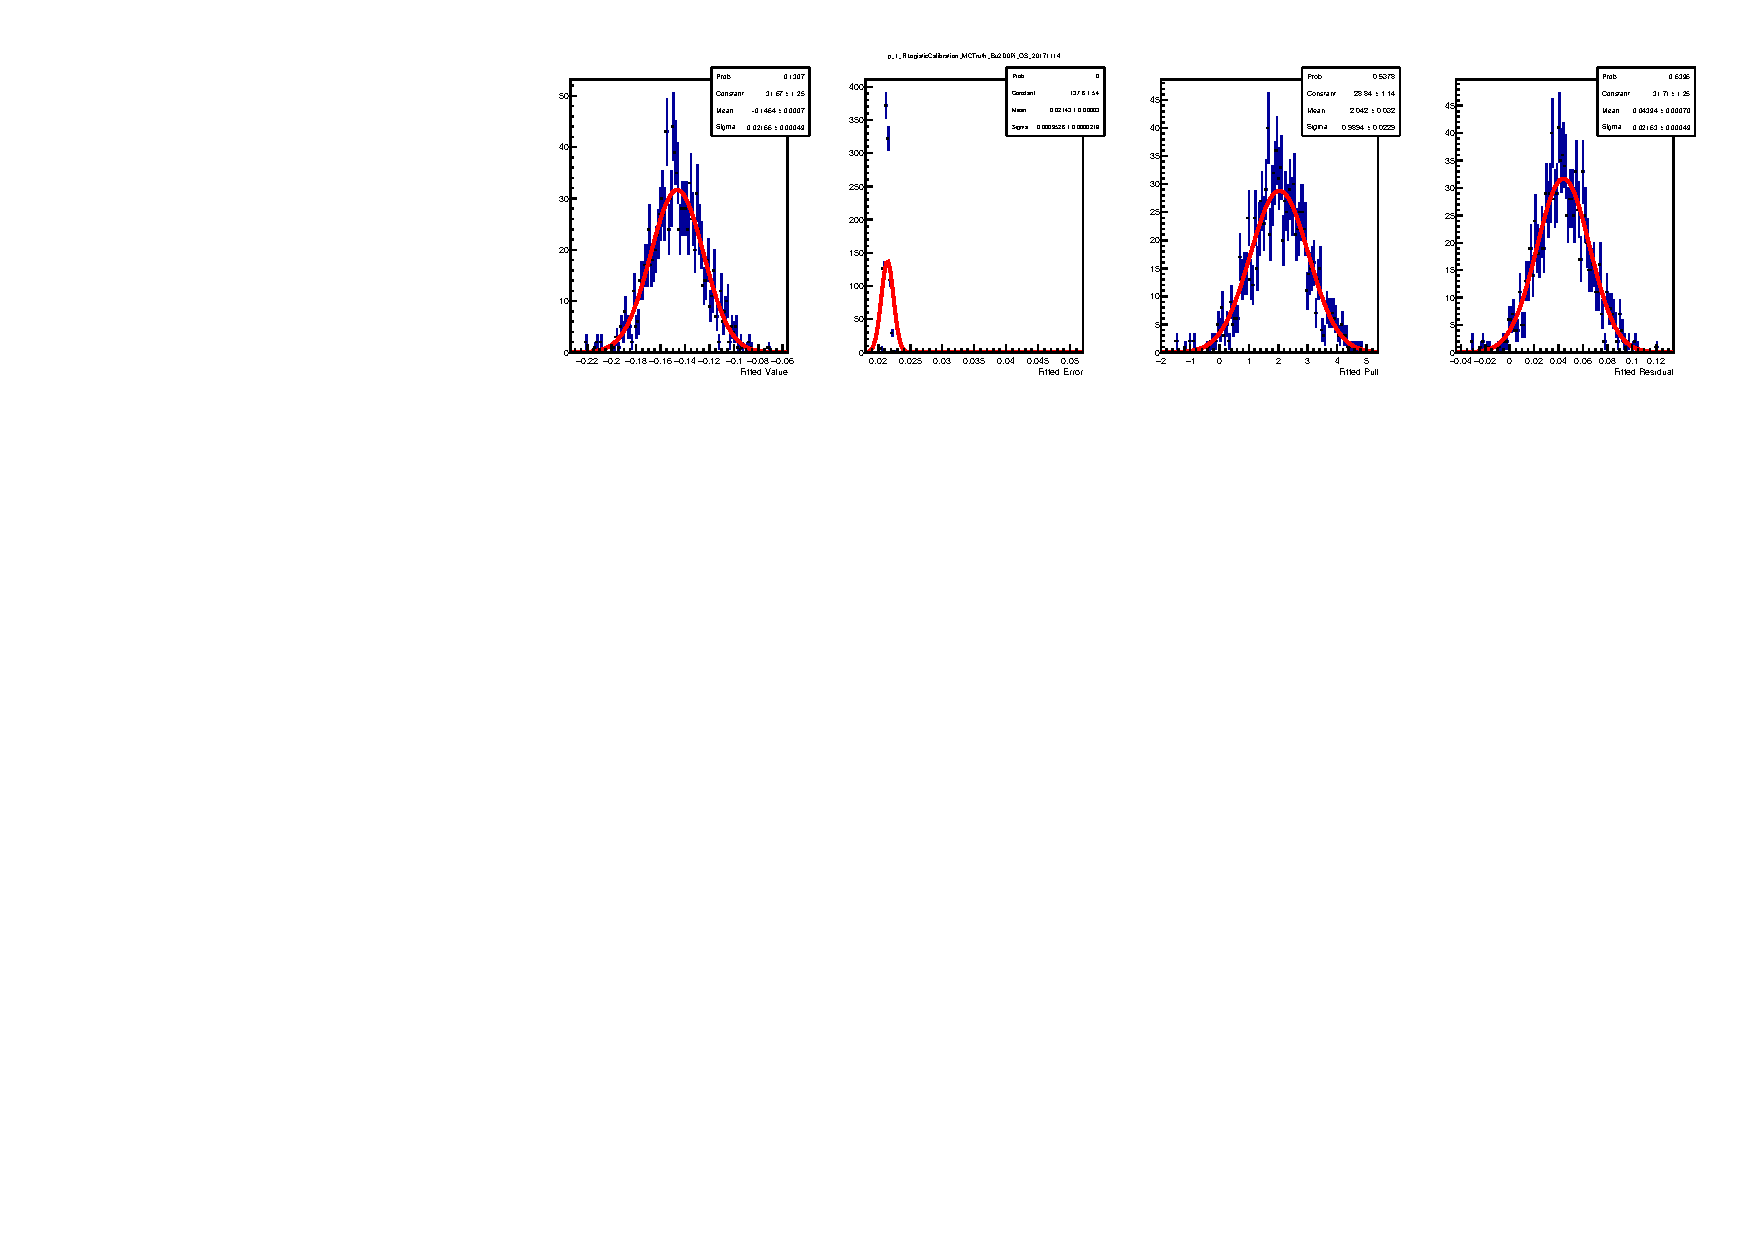
\includegraphics[width=0.8\textwidth]{AA-Appdx-mcbootstrap/figs/1DPullPlot_p_1_RLogisticCalibration_MCTruth_Bu2D0Pi_OS_20171114_SSbarAccAsymmFTFloatDMGammaConstrAllSamples.pdf} \\
    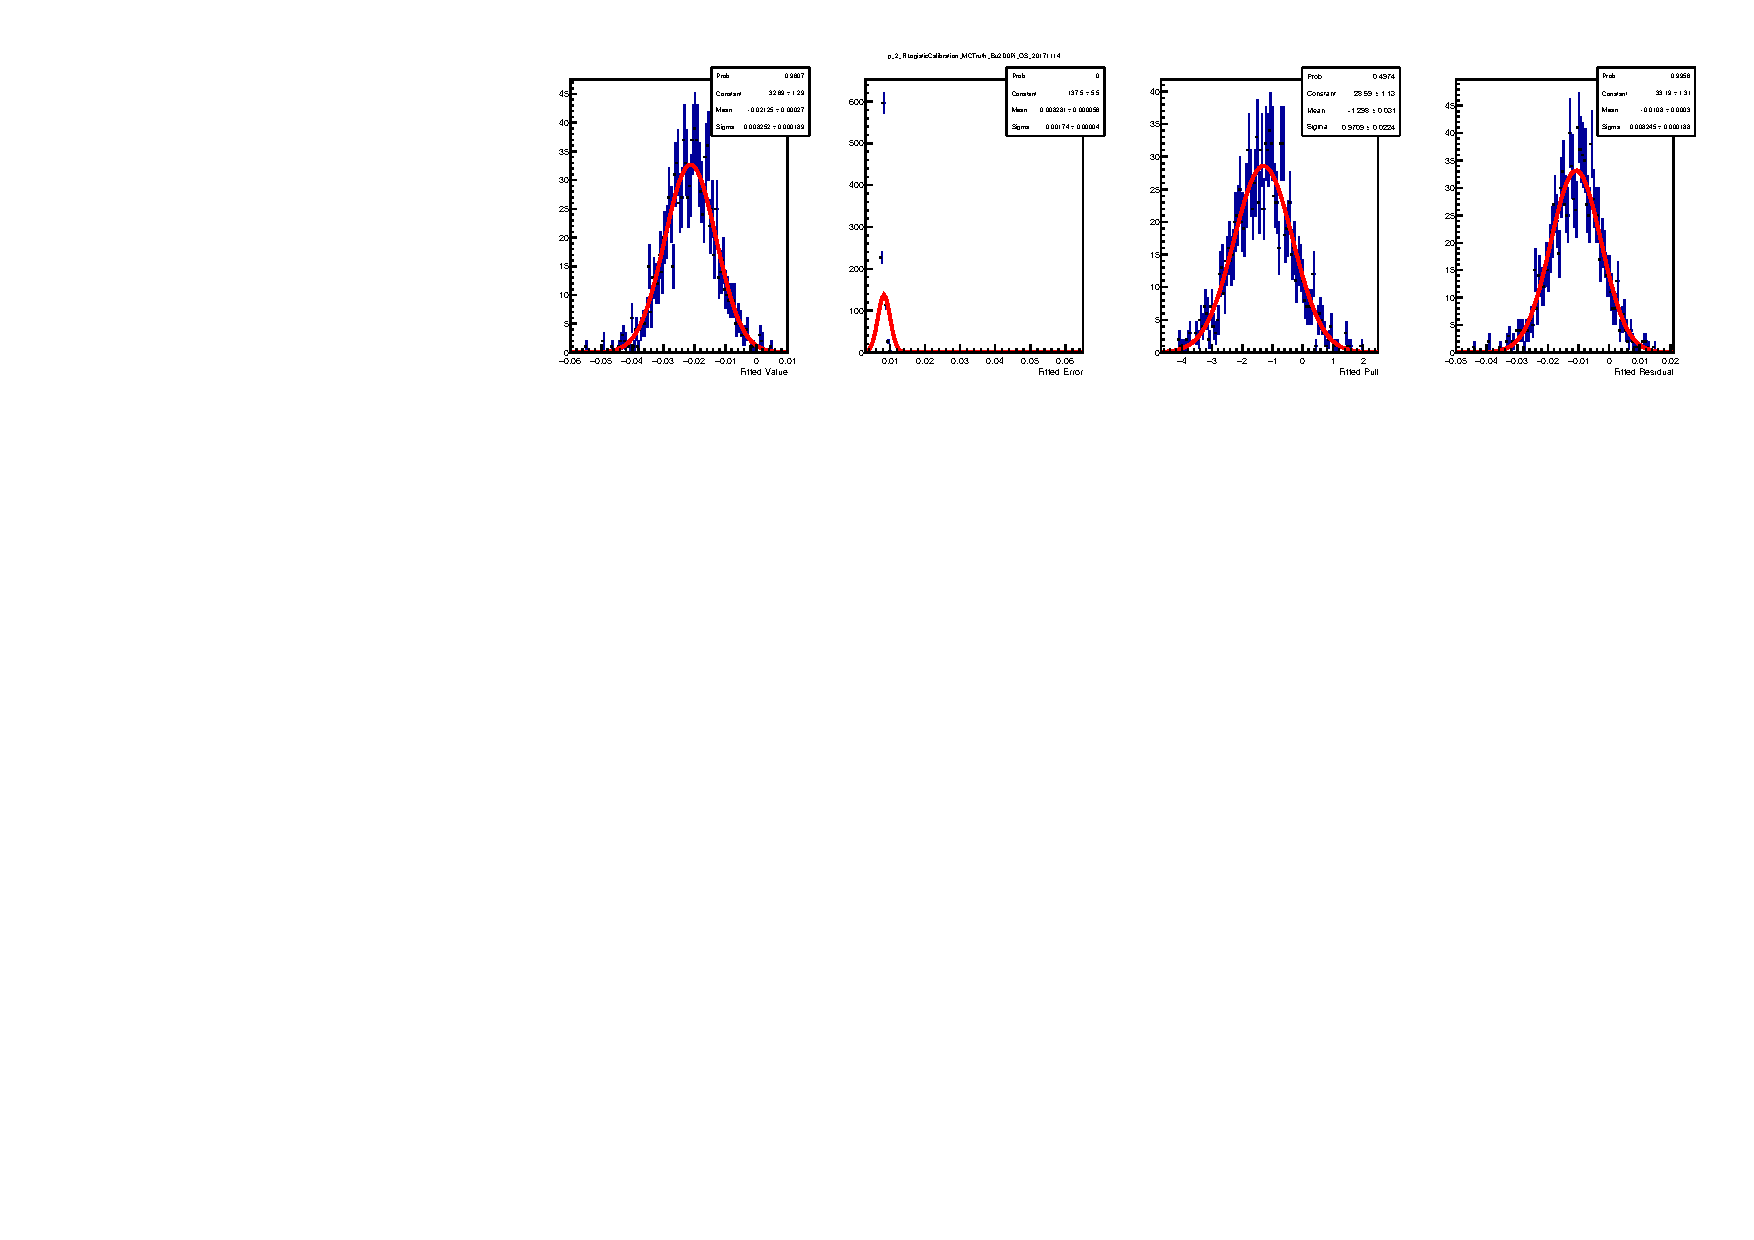
\includegraphics[width=0.8\textwidth]{AA-Appdx-mcbootstrap/figs/1DPullPlot_p_2_RLogisticCalibration_MCTruth_Bu2D0Pi_OS_20171114_SSbarAccAsymmFTFloatDMGammaConstrAllSamples.pdf} \\
    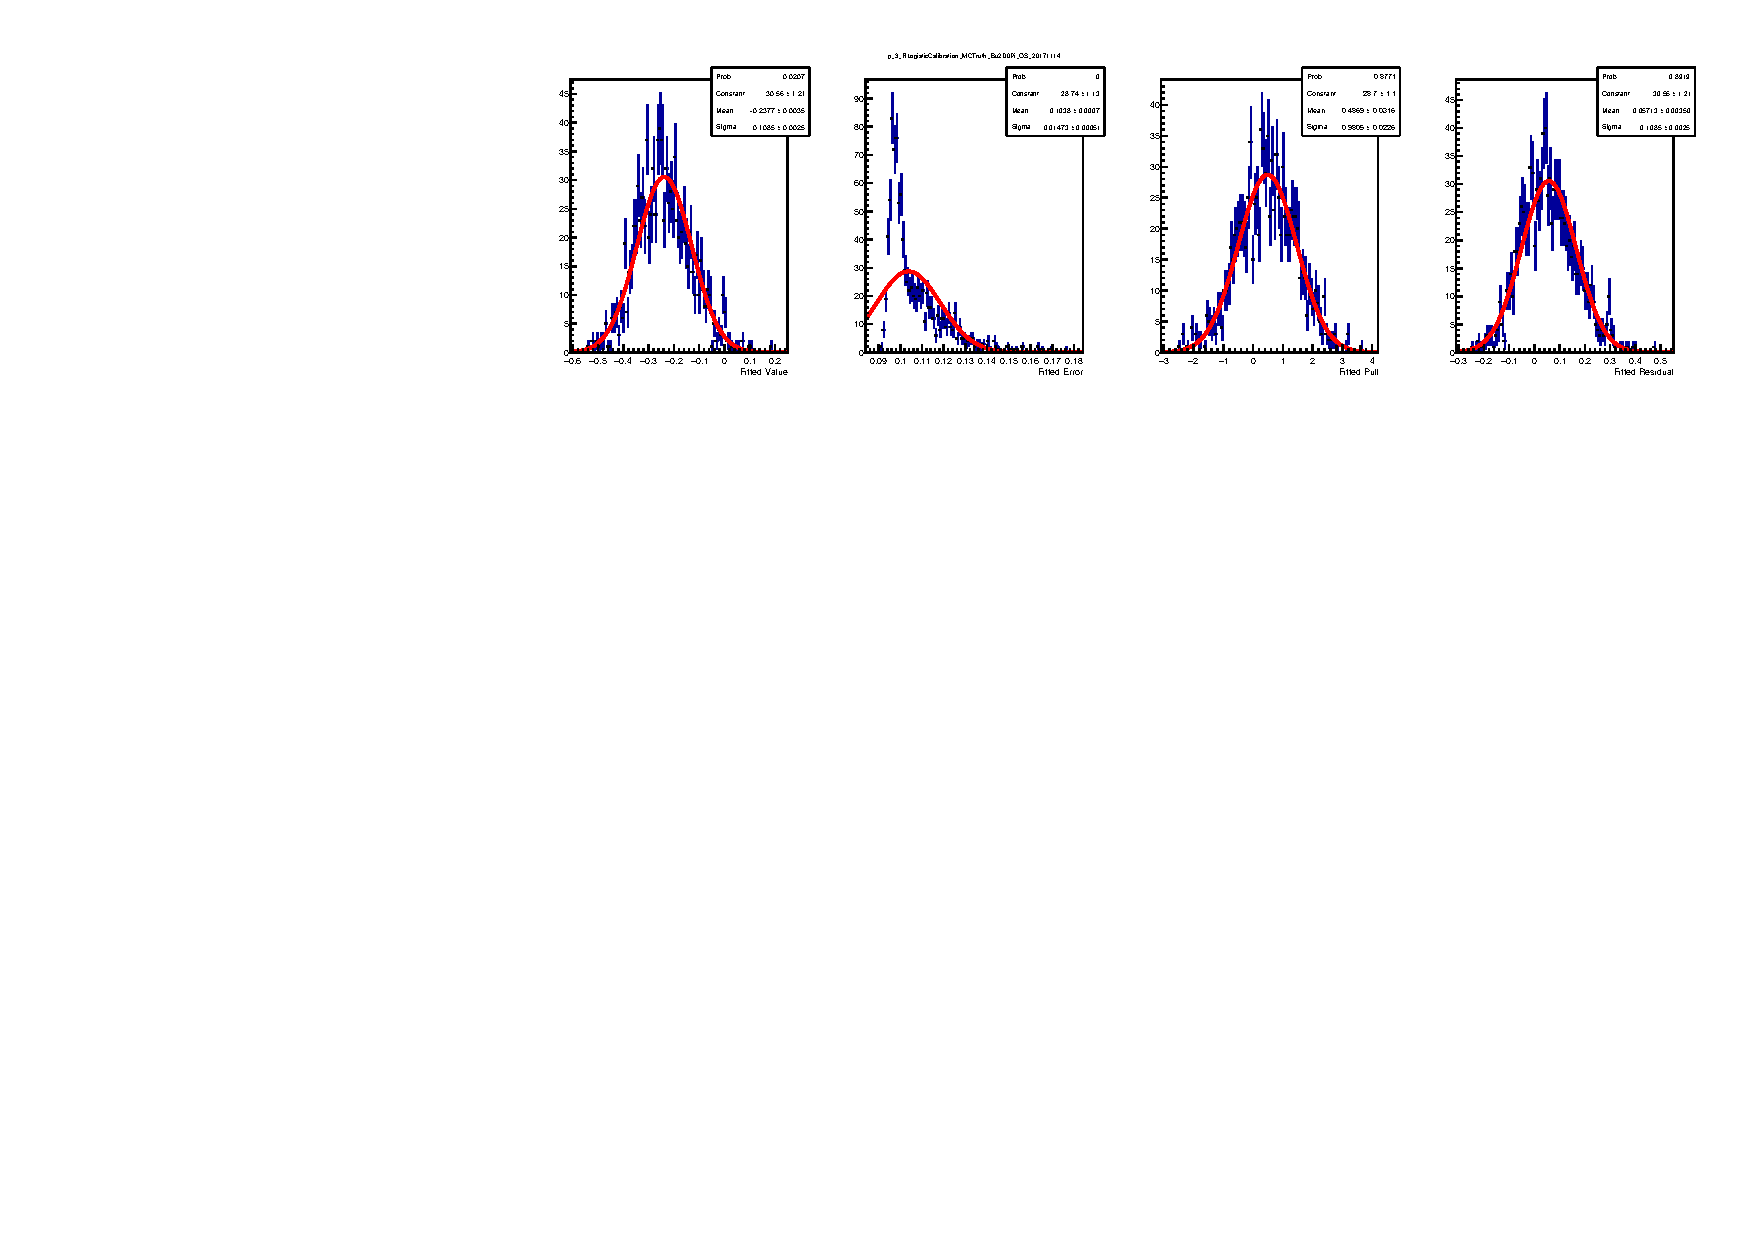
\includegraphics[width=0.8\textwidth]{AA-Appdx-mcbootstrap/figs/1DPullPlot_p_3_RLogisticCalibration_MCTruth_Bu2D0Pi_OS_20171114_SSbarAccAsymmFTFloatDMGammaConstrAllSamples.pdf} \\
    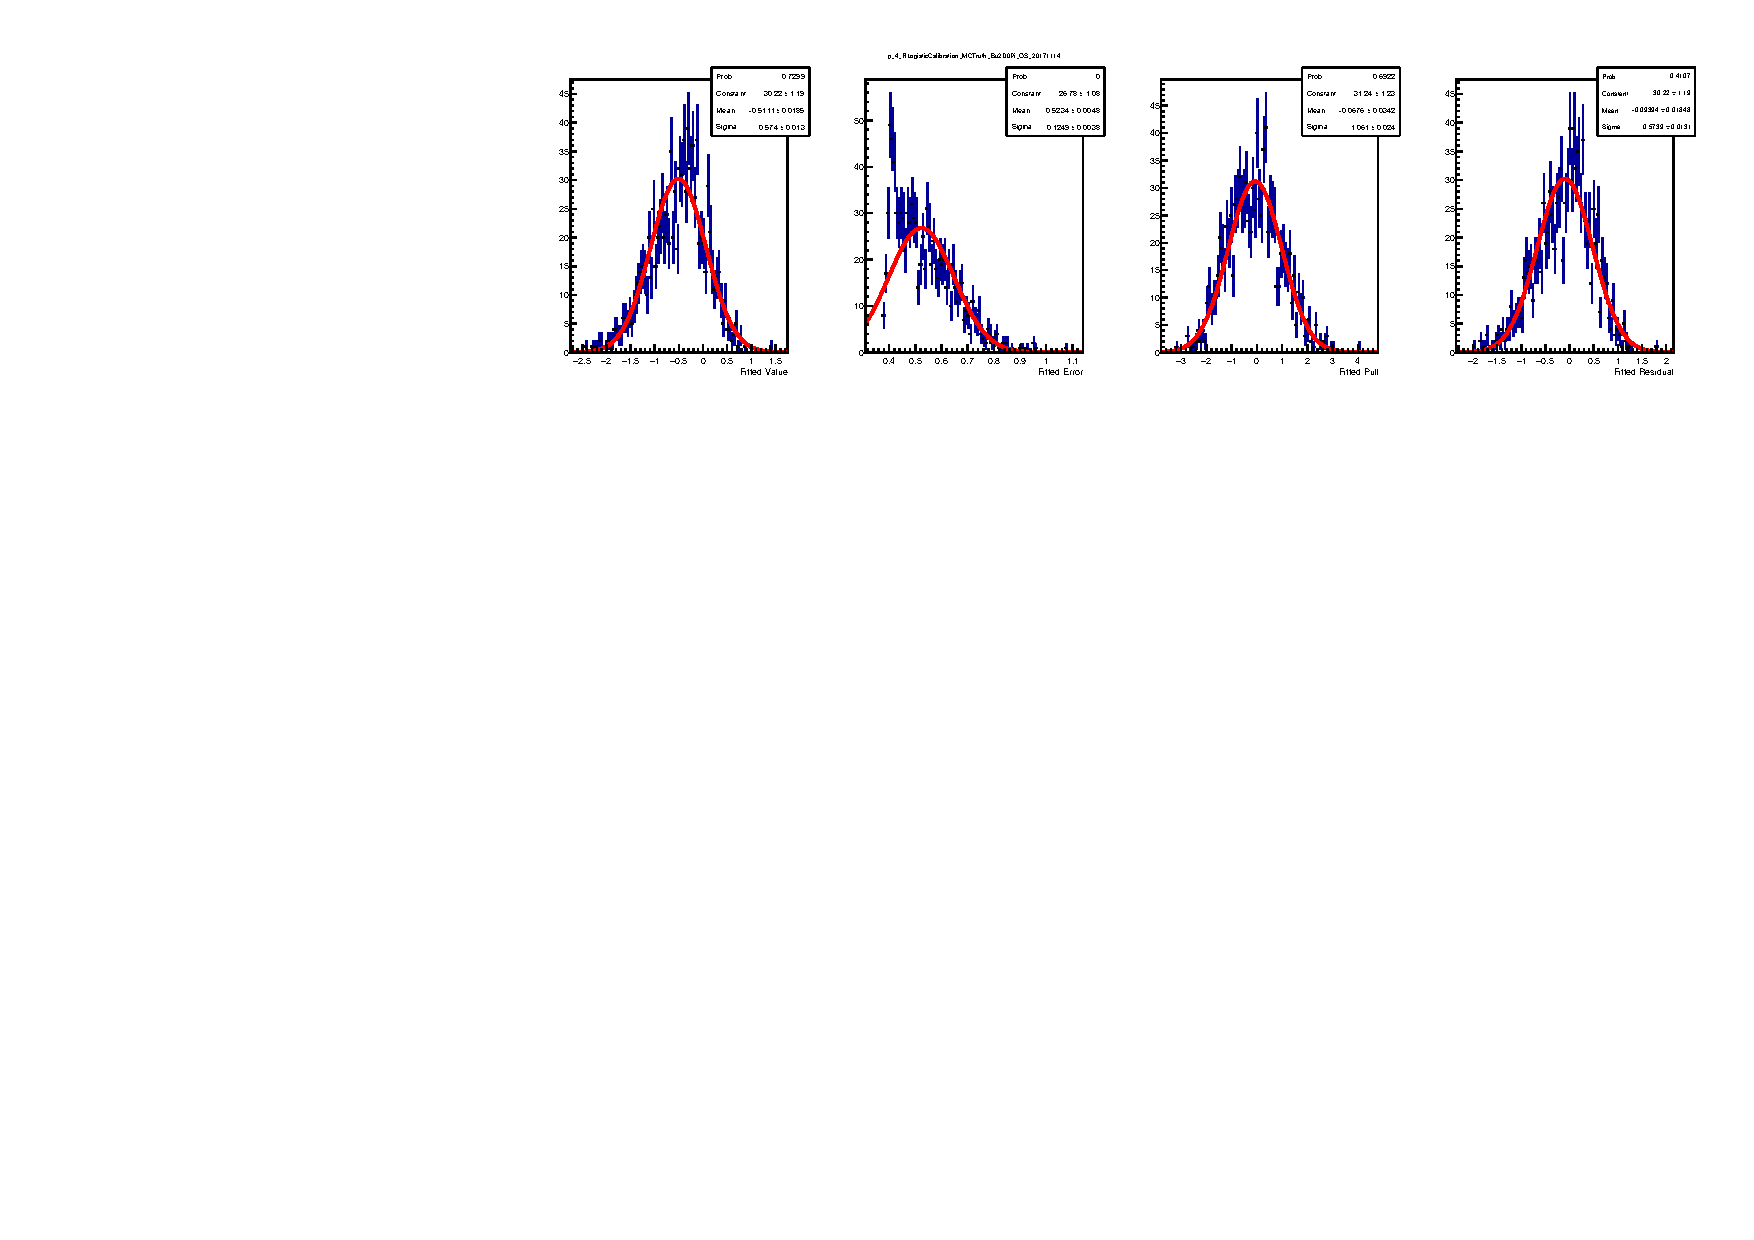
\includegraphics[width=0.8\textwidth]{AA-Appdx-mcbootstrap/figs/1DPullPlot_p_4_RLogisticCalibration_MCTruth_Bu2D0Pi_OS_20171114_SSbarAccAsymmFTFloatDMGammaConstrAllSamples.pdf}
    \end{center}
  \vspace{-2mm}
  \caption{Distributions of the fitted value, error, pull and residual for the OS tagger calibration parameters $p_0^{\rm OS}$, $p_1^{\rm OS}$, $p_2^{\rm OS}$, $p_3^{\rm OS}$, and $p_4^{\rm OS}$ (from top to bottom). Each distribution is fitted with a Gaussian function. The result of the Gaussian fit is shown for the fitted error as well, even though uncertainties are not always Gaussian. Pulls and residuals are computed by taking the values found on the $\Bp\to \Dzb\pip$ Monte Carlo calibration as reference (see Table~\ref{tab:os_calib_portability_mc}).}
  \label{fig:mc_bootstrap_os}
\end{figure}

\begin{figure}[t]
  \begin{center}
    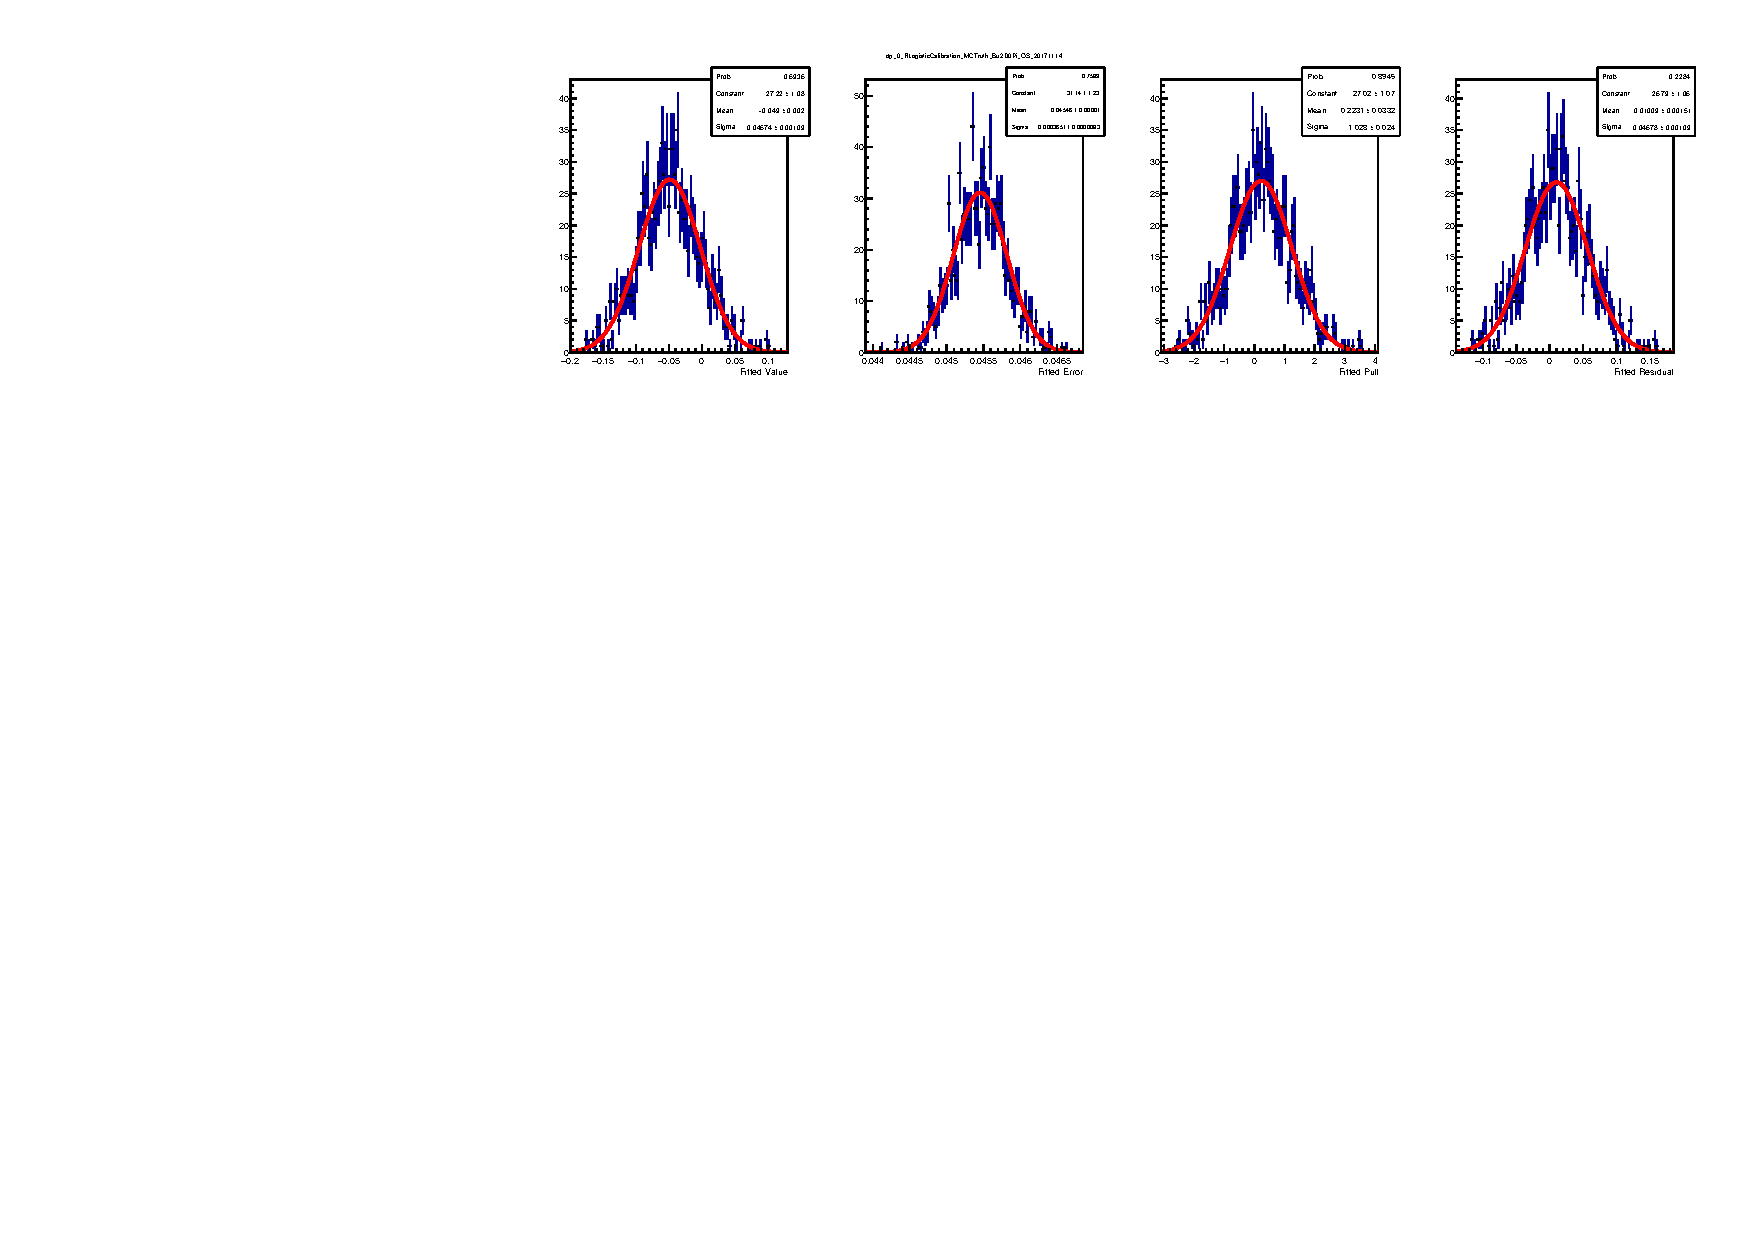
\includegraphics[width=0.8\textwidth]{AA-Appdx-mcbootstrap/figs/1DPullPlot_dp_0_RLogisticCalibration_MCTruth_Bu2D0Pi_OS_20171114_SSbarAccAsymmFTFloatDMGammaConstrAllSamples.pdf} \\
    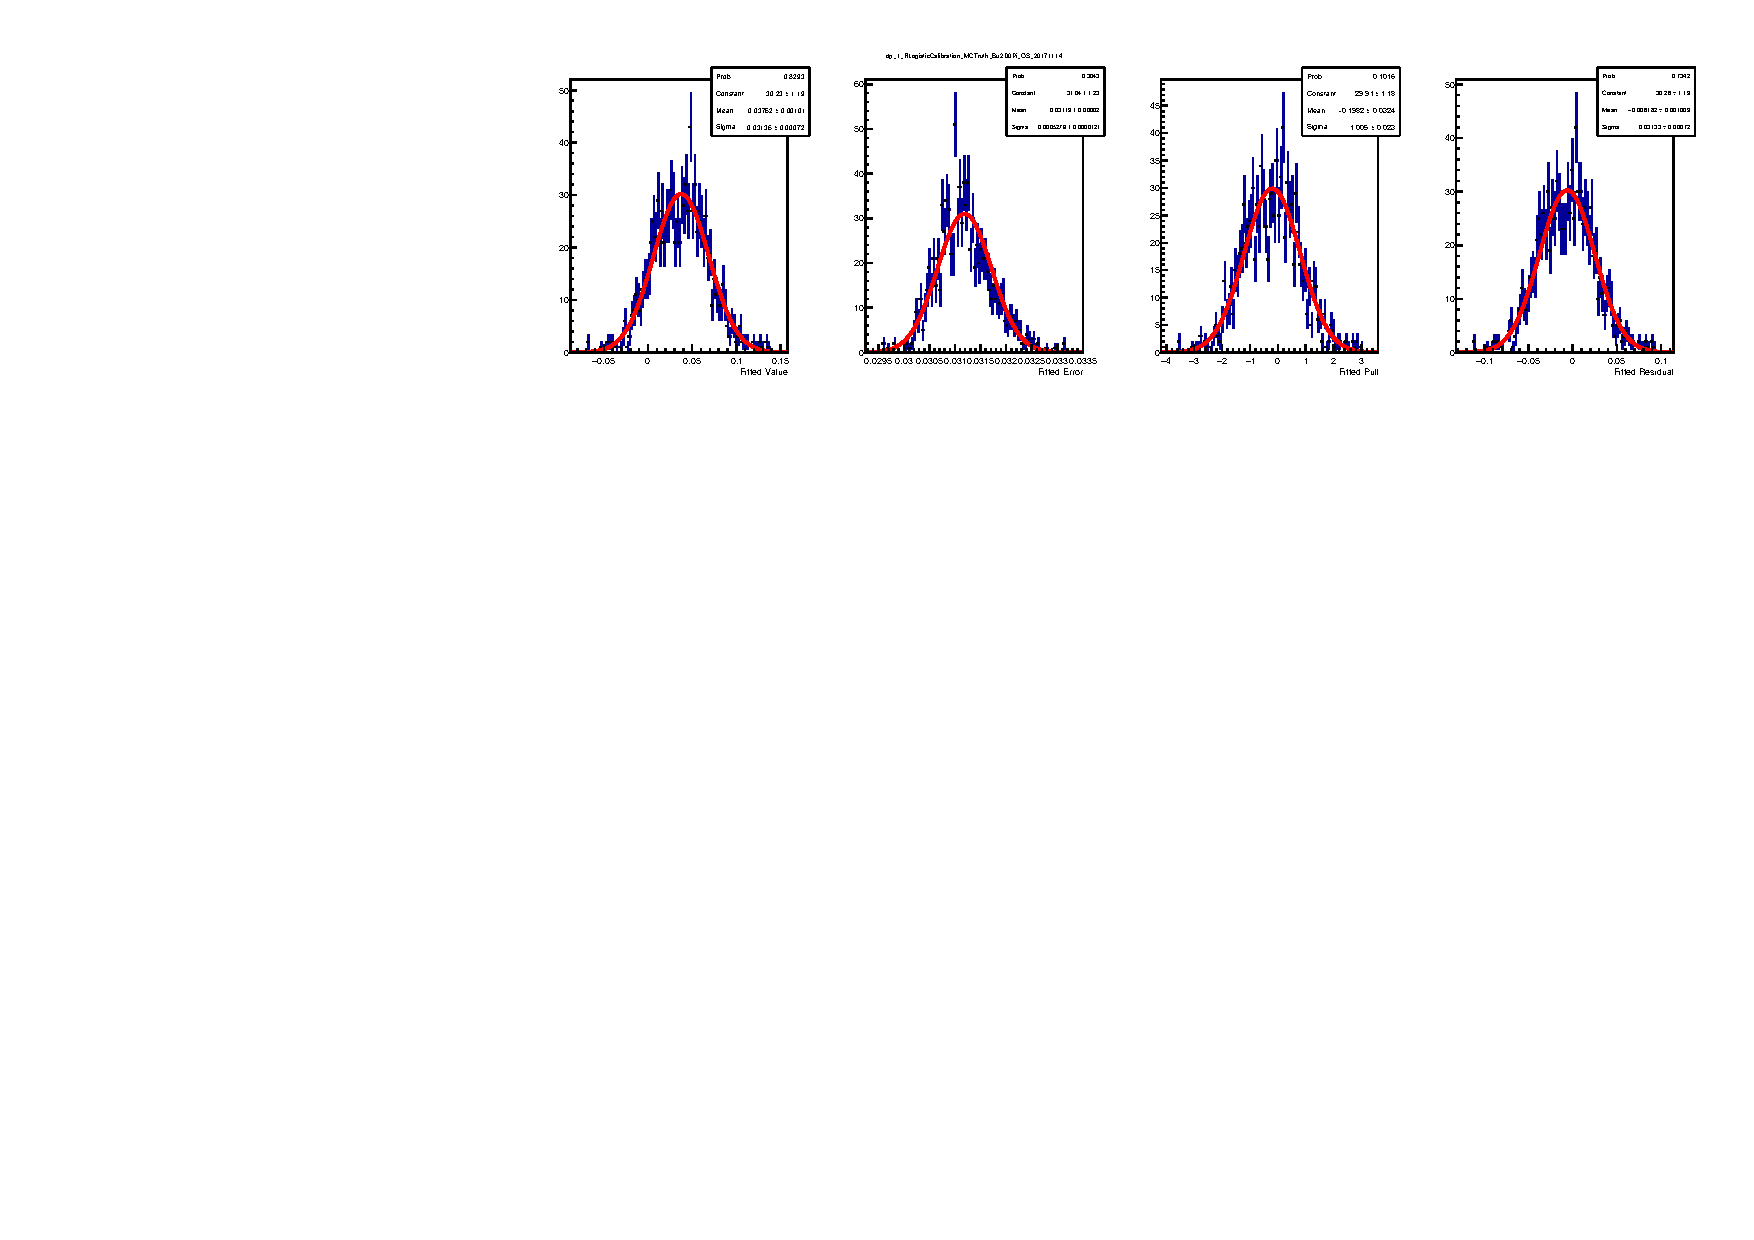
\includegraphics[width=0.8\textwidth]{AA-Appdx-mcbootstrap/figs/1DPullPlot_dp_1_RLogisticCalibration_MCTruth_Bu2D0Pi_OS_20171114_SSbarAccAsymmFTFloatDMGammaConstrAllSamples.pdf} \\
    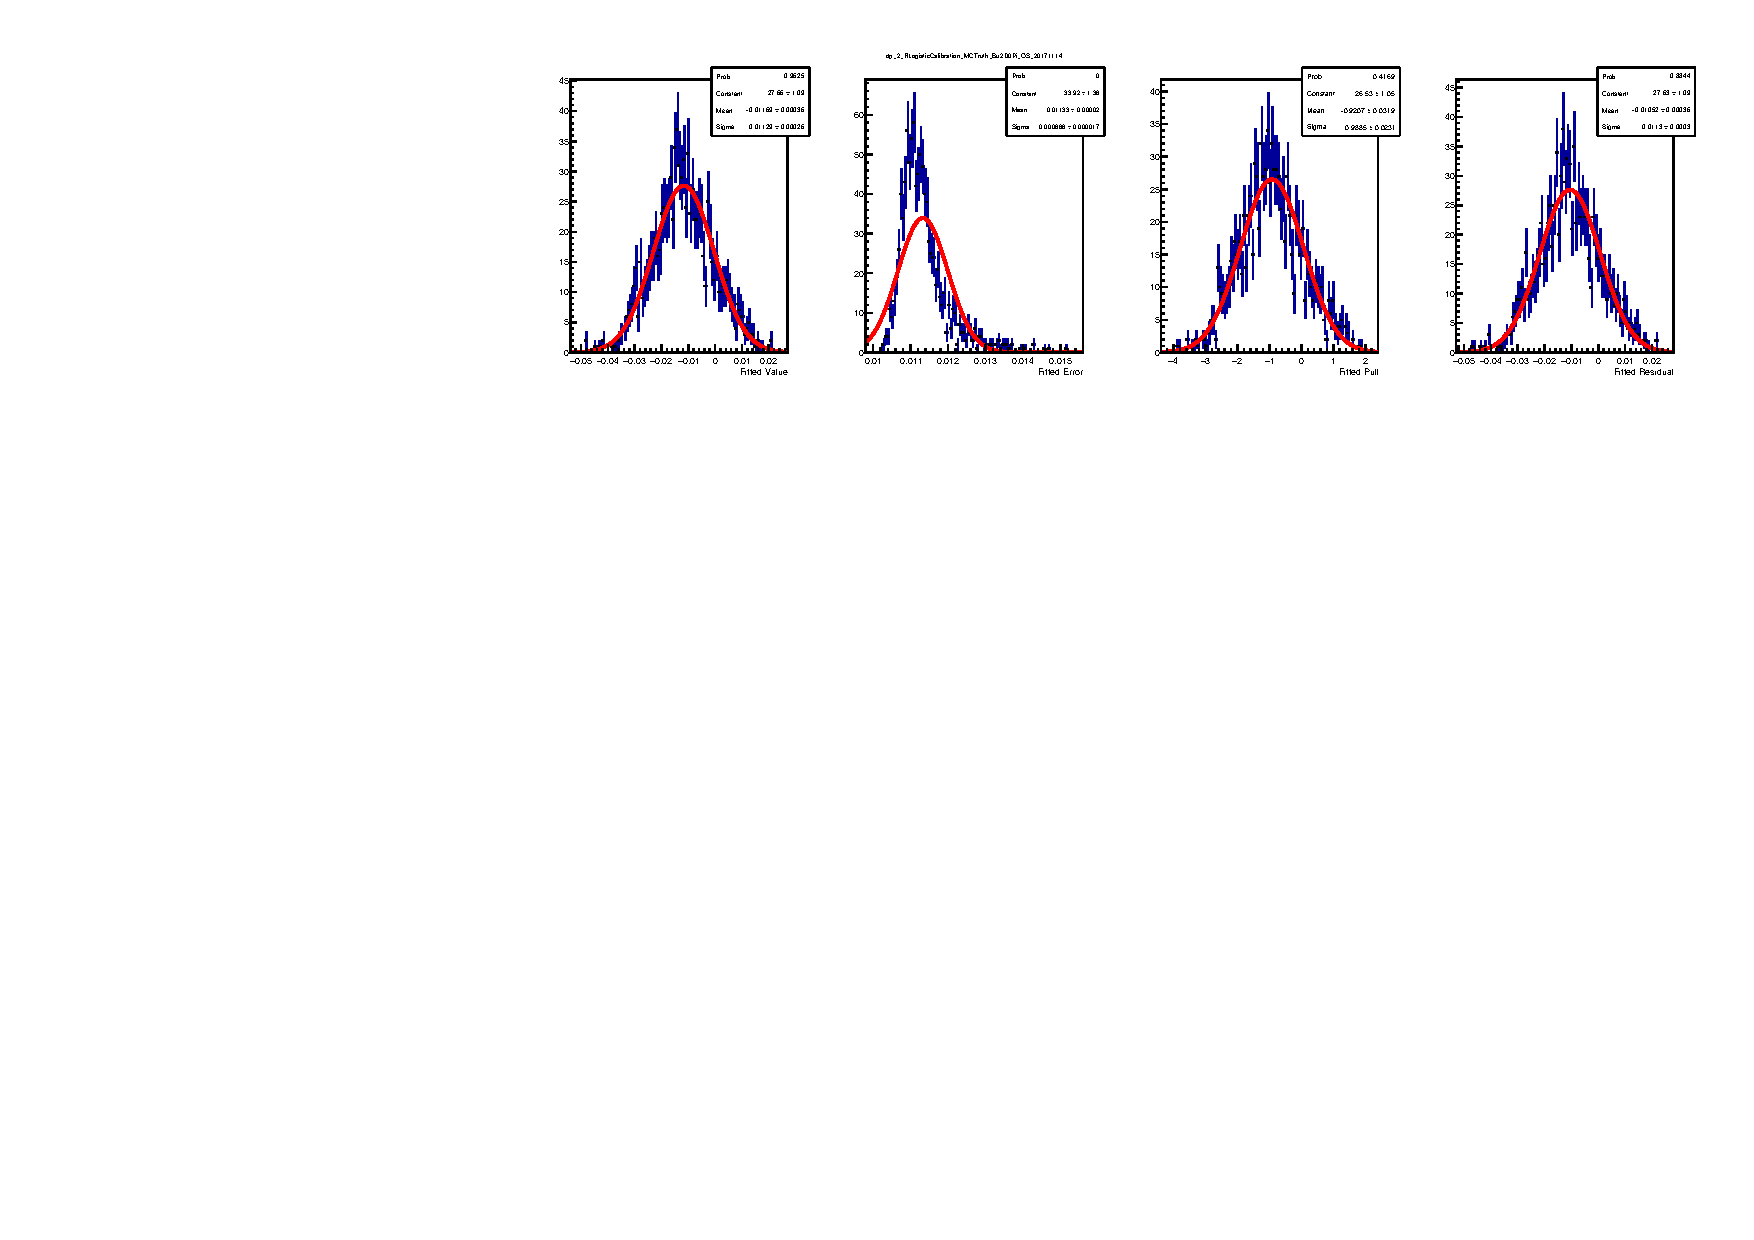
\includegraphics[width=0.8\textwidth]{AA-Appdx-mcbootstrap/figs/1DPullPlot_dp_2_RLogisticCalibration_MCTruth_Bu2D0Pi_OS_20171114_SSbarAccAsymmFTFloatDMGammaConstrAllSamples.pdf} \\
    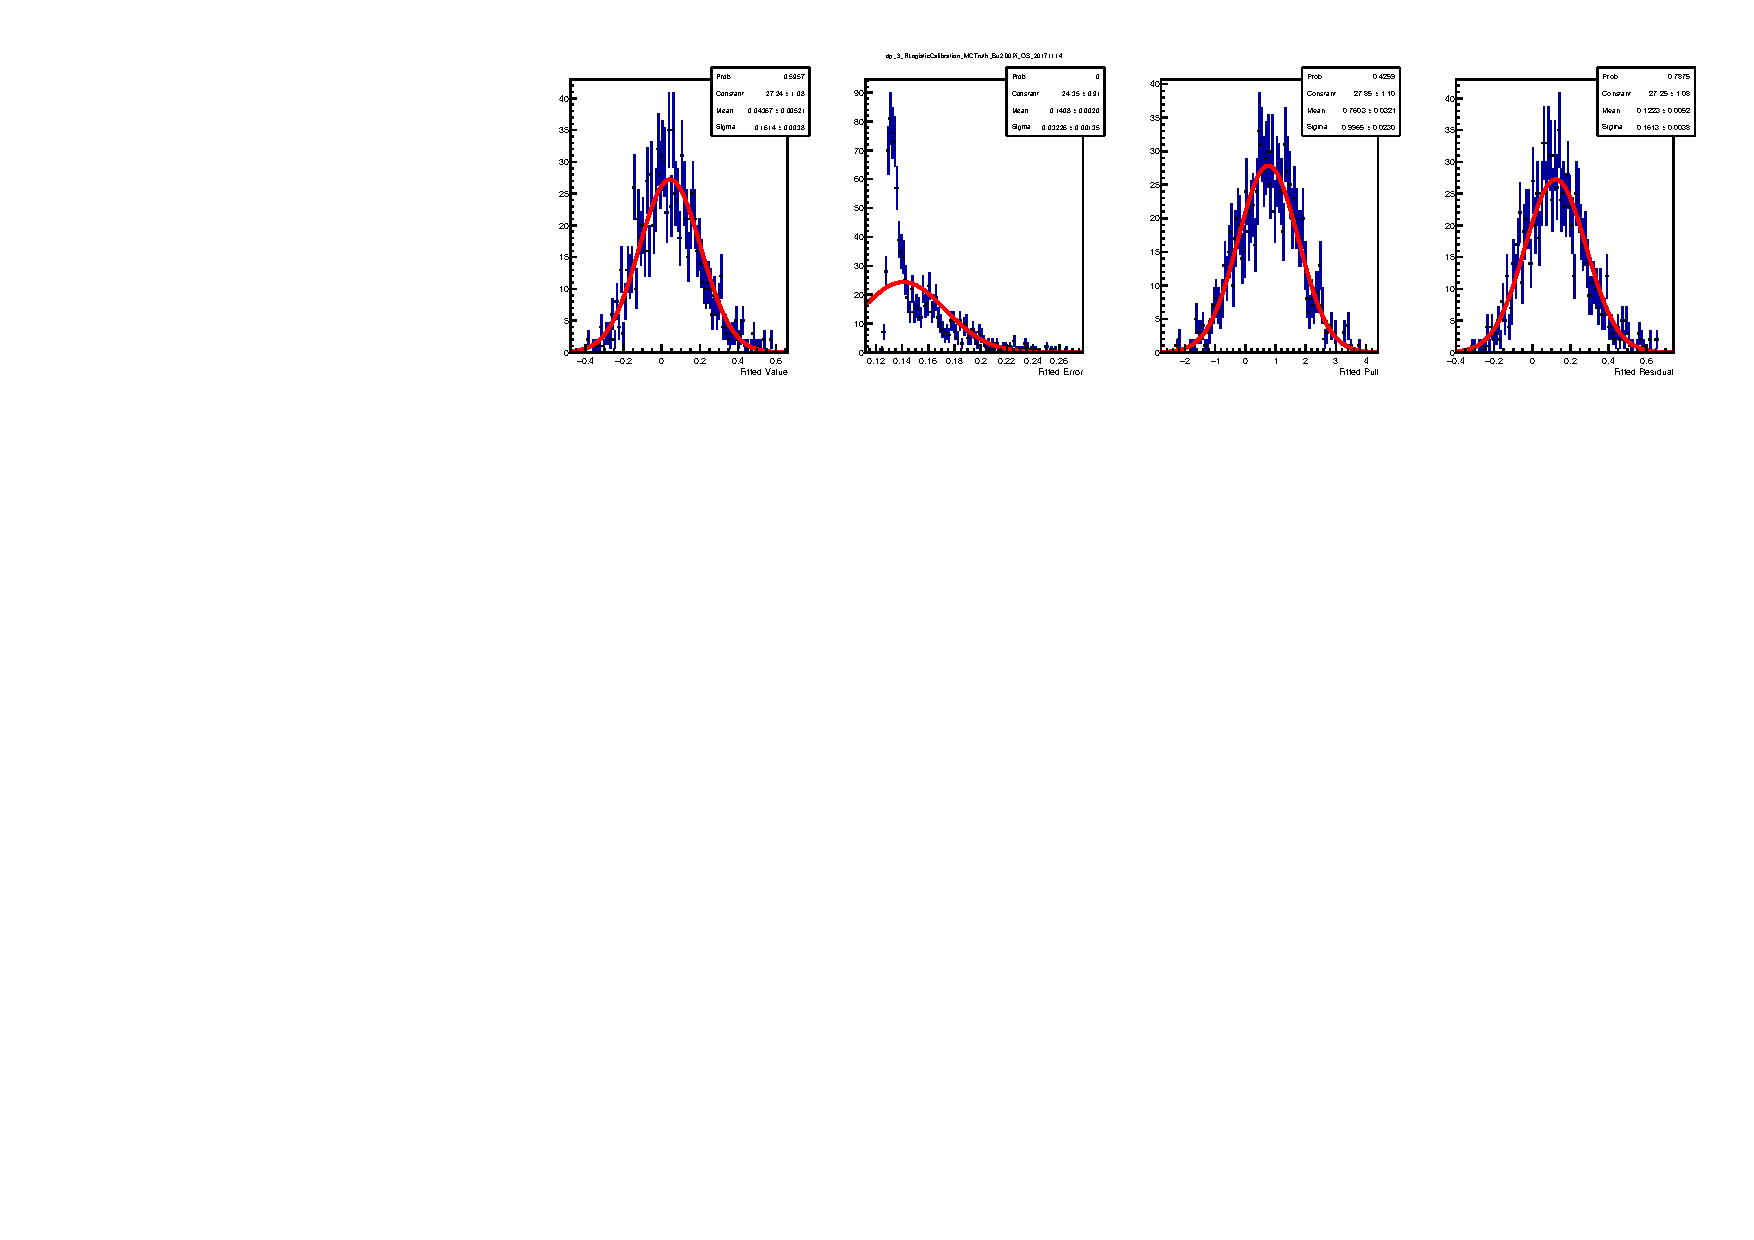
\includegraphics[width=0.8\textwidth]{AA-Appdx-mcbootstrap/figs/1DPullPlot_dp_3_RLogisticCalibration_MCTruth_Bu2D0Pi_OS_20171114_SSbarAccAsymmFTFloatDMGammaConstrAllSamples.pdf} \\
    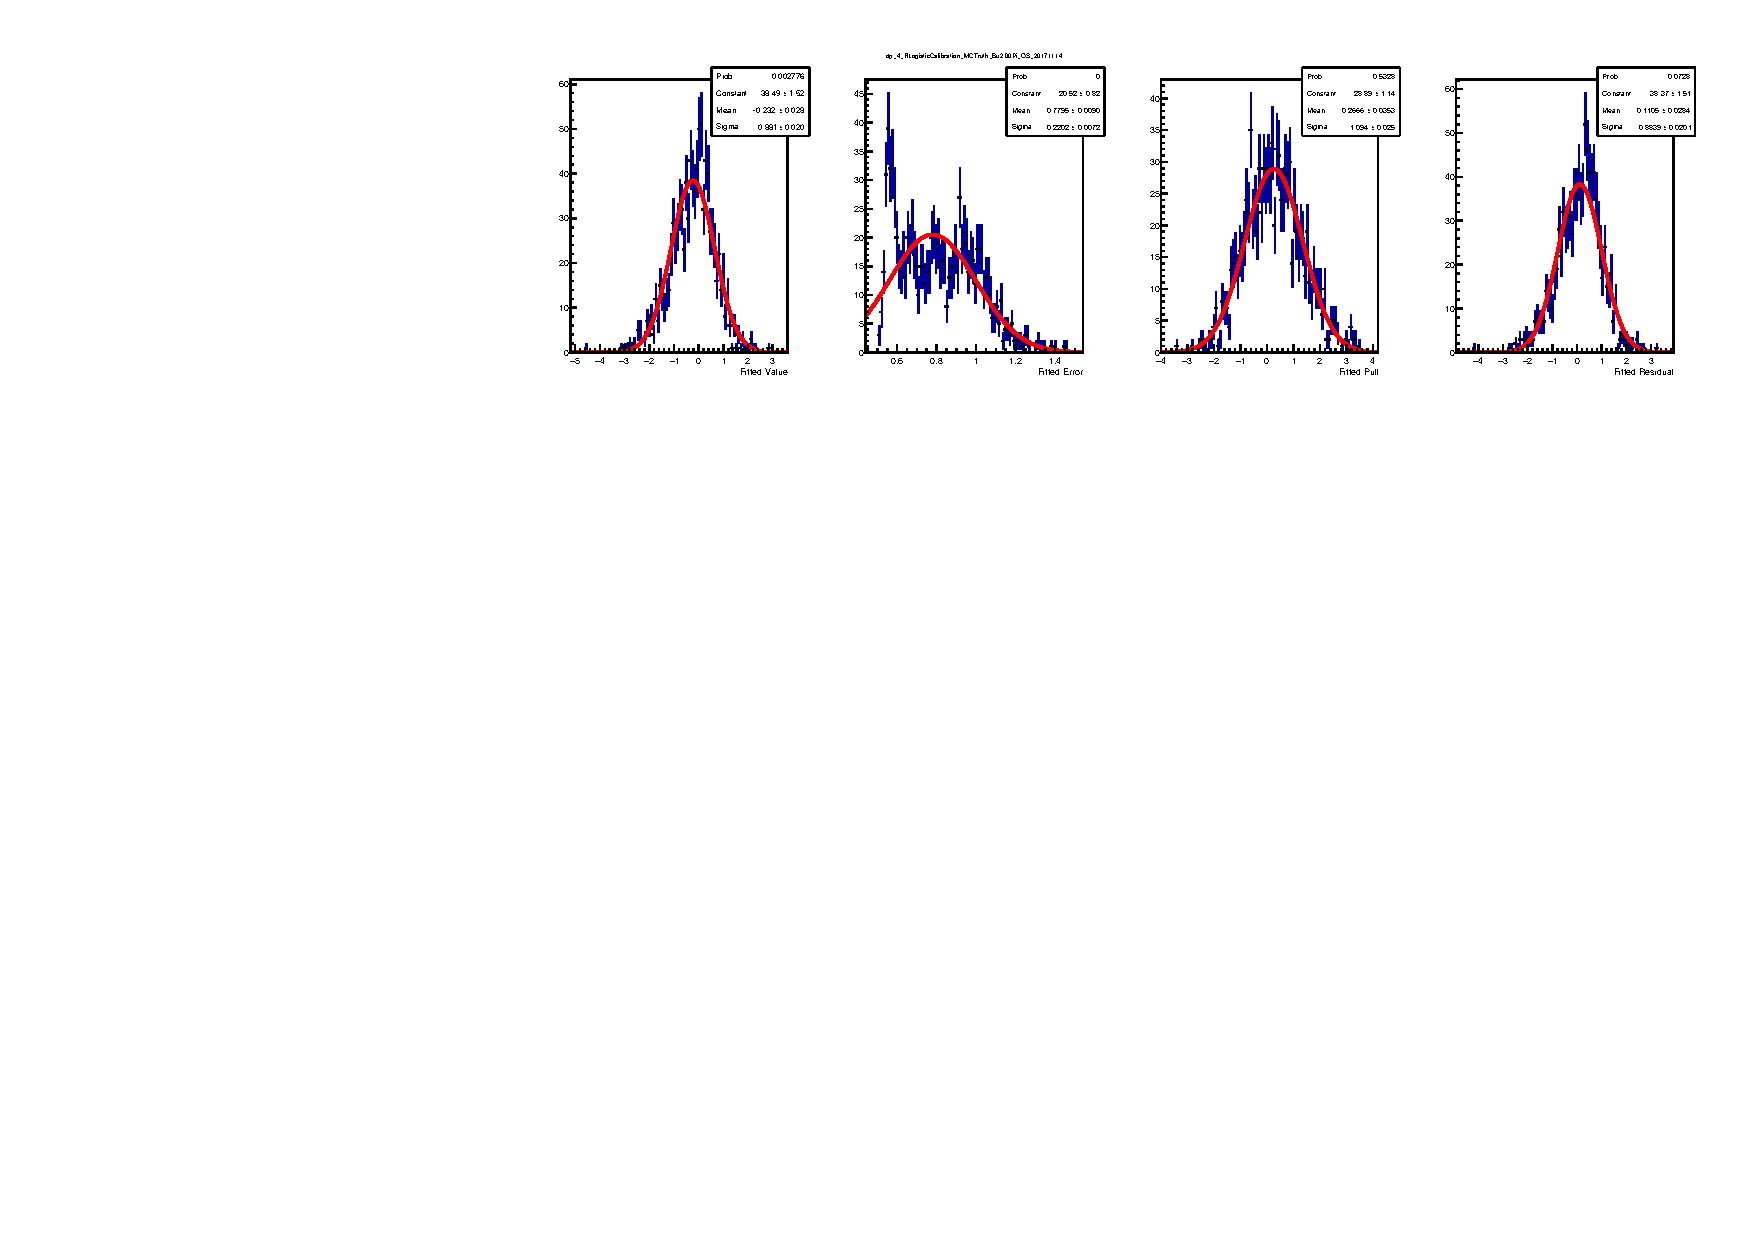
\includegraphics[width=0.8\textwidth]{AA-Appdx-mcbootstrap/figs/1DPullPlot_dp_4_RLogisticCalibration_MCTruth_Bu2D0Pi_OS_20171114_SSbarAccAsymmFTFloatDMGammaConstrAllSamples.pdf} \\
    \end{center}
  \vspace{-2mm}
\caption{Distributions of the fitted value, error, pull and residual for the OS tagger calibration parameters $\Delta p_0^{\rm OS}$, $\Delta p_1^{\rm OS}$, $\Delta p_2^{\rm OS}$, $\Delta p_3^{\rm OS}$, and $\Delta p_4^{\rm OS}$ (from top to bottom). Each distribution is fitted with a Gaussian function. The result of the Gaussian fit is shown for the fitted error as well, even though uncertainties are not always Gaussian. Pulls and residuals are computed by taking the values found on the $\Bp\to \Dzb\pip$ Monte Carlo calibration as reference (see Table~\ref{tab:os_calib_portability_mc}).}
  \label{fig:mc_bootstrap_deltaos}
\end{figure}
